\chapter{Experimental Results and Discussion} \label{chap:results}

\section{Grader Performance} \label{sec:grader_performance}
This section presents the performance of the grader models trained with the three different features: feature, text, and audio. Accurate models set foundation for the subsequent sections on bias detection and analysis.

The accuracy of the three models, both calibrated and uncalibrated, is presented in Table \ref{tab:model_accuracy}. The table shows the Root Mean Square Error (RMSE), Pearson Correlation Coefficient (PCC), and the percentage of predictions that are less than 0.5 ($< 0.5$) and 1.0 ($< 1$) from the ground truth. The coefficients for the linear calibration of the three models are presented in Table \ref{tab:linear_regression_coefficients} as a reference. All the models perform decently well with similar results for the metric values, with all the RMSE approximately in the range of $0.6$ to $0.7$, PCC in $0.8$ to $0.9$ $< 0.5$ in $55-60\%$, and $< 1$ in $80-90\%$. All the calibrated models only show a slight improvement in the performance. Overall, the results indicate that the models are capable of predicting the scores with reasonable accuracy, hence reliable for CAV extraction.
\begin{table}[H]
    \centering
    \begin{tabular}{|l|c|c|c|c|c|}
        \hline
        \multicolumn{2}{|l|}{}                                  & \textbf{RMSE}         & \textbf{PCC} & \textbf{\textless 0.5} & \textbf{\textless 1}        \\ \hline
        \multicolumn{1}{|l|}{\multirow{2}{*}{\textbf{Feature}}} & \textbf{Uncalibrated} & 0.694        & 0.821                  & 55.3                 & 83.4 \\ \cline{2-6}
        \multicolumn{1}{|l|}{}                                  & \textbf{Calibrated}   & 0.638        & 0.821                  & 56.6                 & 87.9 \\ \hline
        \multicolumn{1}{|l|}{\multirow{2}{*}{\textbf{Text}}}    & \textbf{Uncalibrated} & 0.678        & 0.837                  & 55.6                 & 84.8 \\ \cline{2-6}
        \multicolumn{1}{|l|}{}                                  & \textbf{Calibrated}   & 0.627        & 0.837                  & 58.1                 & 88.2 \\ \hline
        \multicolumn{1}{|l|}{\multirow{2}{*}{\textbf{Audio}}}   & \textbf{Uncalibrated} & 0.671        & 0.853                  & 57.3                 & 85.4 \\ \cline{2-6}
        \multicolumn{1}{|l|}{}                                  & \textbf{Calibrated}   & 0.598        & 0.853                  & 61.1                 & 89.0 \\ \hline
    \end{tabular}
    \caption{Model accuracy for the three models, both calibrated and uncalibrated.}
    \label{tab:model_accuracy}
\end{table}

\begin{table}[H]
    \centering
    \begin{tabular}{|l|c|c|}
        \hline
        \textbf{}        & \textbf{Slope (m)} & \textbf{Intercept (c)} \\ \hline
        \textbf{Feature} & 1.42               & -1.45                  \\ \hline
        \textbf{Text}    & 1.19               & -0.80                  \\ \hline
        \textbf{Audio}   & 1.14               & -0.75                  \\ \hline
    \end{tabular}
    \caption{Linear calibration coefficients for the three models}
    \label{tab:linear_regression_coefficients}
\end{table}

\section{Bias Detection} \label{sec:bias_detection}
This section presents the results of bias detection performed on text-based, feature-based and audio-based models. Section \ref{sec:cav_accuracy} presents the accuracy of the CAV extracted, and Section \ref{sec:gradient_distance} examines the bias measurement results through gradient distance. Finally, section \ref{sec:model_biasing} discusses the bias measurement results on the biased version of the three models.

\subsection{CAV Accuracy} \label{sec:cav_accuracy}
The accuracy of the CAV extracted using the first layer of activations from the three models is presented in Table \ref{tab:CAV_accuracy_combined}, with the data averaged across all seeds. The table shows the accuracy of the CAV in differentiating positive and negative training data for each concept, both with and without balanced weighting. Those with accuracy less than 60\% are highlighted in red. In addition, the percentage of positive targets for each concept from the training data is shown in Table \ref{tab:pos_target}, with which the training data is used for extracting and evaluating the CAV.

\begin{table}[H]
    \centering
    \begin{tabular}{|c|c|cc|cc|cc|}
        \hline
        \multirow{2}{*}{} & \multirow{2}{*}{\textbf{Concept}} & \multicolumn{2}{c|}{\textbf{Feature}}                     & \multicolumn{2}{c|}{\textbf{Text}}   & \multicolumn{2}{c|}{\textbf{Audio}}                                                                                                                                             \\ \cline{3-8}
                          &                                   & \multicolumn{1}{c|}{\textbf{+ve}}                         & \textbf{-ve}                         & \multicolumn{1}{c|}{\textbf{+ve}}                         & \textbf{-ve}                         & \multicolumn{1}{c|}{\textbf{+ve}}                         & \textbf{-ve}     \\ \hline
        \multirow{7}{*}{\rotatebox{90}{\scriptsize \textbf{No weighting}}}
                          & $\geq$ C1                         & \multicolumn{1}{c|}{\cellcolor{red!15}{$0_{\pm 0}$}}      & $100_{\pm 0}$                        & \multicolumn{1}{c|}{\cellcolor{red!15}{$0_{\pm 0}$}}      & $100_{\pm 0}$                        & \multicolumn{1}{c|}{\cellcolor{red!15}{$0_{\pm 0}$}}      & $100_{\pm 0}$    \\
                          & $\geq$ B2                         & \multicolumn{1}{c|}{\cellcolor{red!15}{$51.0_{\pm 1.4}$}} & $95.2_{\pm 0.1}$                     & \multicolumn{1}{c|}{\cellcolor{red!15}{$49.5_{\pm 1.9}$}} & $95.5_{\pm 0.2}$                     & \multicolumn{1}{c|}{\cellcolor{red!15}{$54.0_{\pm 0.7}$}} & $95.6_{\pm 0.1}$ \\
                          & $\leq$ A2                         & \multicolumn{1}{c|}{\cellcolor{red!15}{$52.6_{\pm 1.4}$}} & $92.9_{\pm 0.2}$                     & \multicolumn{1}{c|}{\cellcolor{red!15}{$56.9_{\pm 1.6}$}} & $93.5_{\pm 0.4}$                     & \multicolumn{1}{c|}{\cellcolor{red!15}{$58.9_{\pm 0.0}$}} & $93.1_{\pm 0.0}$ \\ \cline{2-8}
                          & Thai                              & \multicolumn{1}{c|}{\cellcolor{red!15}{$52.3_{\pm 4.6}$}} & $93.1_{\pm 0.8}$                     & \multicolumn{1}{c|}{\cellcolor{red!15}{$44.6_{\pm 8.7}$}} & $95.4_{\pm 0.4}$                     & \multicolumn{1}{c|}{$91.0_{\pm 0.0}$}                     & $97.9_{\pm 0.0}$ \\
                          & Spanish                           & \multicolumn{1}{c|}{$75.1_{\pm 0.4}$}                     & $79.9_{\pm 0.7}$                     & \multicolumn{1}{c|}{$72.2_{\pm 4.6}$}                     & $77.5_{\pm 5.4}$                     & \multicolumn{1}{c|}{$88.2_{\pm 0.0}$}                     & $90.7_{\pm 0.0}$ \\ \cline{2-8}
                          & Young                             & \multicolumn{1}{c|}{$77.4_{\pm 0.4}$}                     & \cellcolor{red!15}{$52.2_{\pm 0.5}$} & \multicolumn{1}{c|}{$78.8_{\pm 1.7}$}                     & \cellcolor{red!15}{$54.1_{\pm 1.6}$} & \multicolumn{1}{c|}{$80.5_{\pm 0.3}$}                     & $72.6_{\pm 0.7}$ \\ \cline{2-8}
                          & Male                              & \multicolumn{1}{c|}{\cellcolor{red!15}{$47.8_{\pm 2.0}$}} & $75.6_{\pm 0.6}$                     & \multicolumn{1}{c|}{\cellcolor{red!15}{$30.8_{\pm 9.1}$}} & $85.1_{\pm 4.8}$                     & \multicolumn{1}{c|}{$94.4_{\pm 0.0}$}                     & $96.5_{\pm 0.0}$ \\ \hline
        \multirow{7}{*}{\rotatebox{90}{\scriptsize \textbf{Balanced weighting}}}
                          & $\geq$ C1                         & \multicolumn{1}{c|}{$94.3_{\pm 1.0}$}                     & $85.0_{\pm 0.3}$                     & \multicolumn{1}{c|}{$99.0_{\pm 0.9}$}                     & \cellcolor{red!15}{$58.3_{\pm 1.7}$} & \multicolumn{1}{c|}{$98.8_{\pm 0}$}                       & $83.1_{\pm 1.4}$ \\
                          & $\geq$ B2                         & \multicolumn{1}{c|}{$84.4_{\pm 0.3}$}                     & $79.0_{\pm 0.3}$                     & \multicolumn{1}{c|}{$87.5_{\pm 0.9}$}                     & $76.1_{\pm 1.7}$                     & \multicolumn{1}{c|}{$86.2_{\pm 0.2}$}                     & $80.2_{\pm 0.1}$ \\
                          & $\leq$ A2                         & \multicolumn{1}{c|}{$86.5_{\pm 0.2}$}                     & $76.0_{\pm 0.6}$                     & \multicolumn{1}{c|}{$87.0_{\pm 0.5}$}                     & $78.9_{\pm 0.6}$                     & \multicolumn{1}{c|}{$87.1_{\pm 0.2}$}                     & $78.5_{\pm 0.1}$ \\ \cline{2-8}
                          & Thai                              & \multicolumn{1}{c|}{$86.2_{\pm 0.9}$}                     & $76.3_{\pm 0.6}$                     & \multicolumn{1}{c|}{$72.2_{\pm 19.9}$}                    & $70.1_{\pm 22.5}$                    & \multicolumn{1}{c|}{$97.2_{\pm 0.0}$}                     & $94.2_{\pm 0.6}$ \\
                          & Spanish                           & \multicolumn{1}{c|}{$79.4_{\pm 0.3}$}                     & $75.8_{\pm 1.1}$                     & \multicolumn{1}{c|}{$79.7_{\pm 2.6}$}                     & $71.0_{\pm 7.1}$                     & \multicolumn{1}{c|}{$91.1_{\pm 0.5}$}                     & $88.7_{\pm 0.3}$ \\ \cline{2-8}
                          & Young                             & \multicolumn{1}{c|}{$74.0_{\pm 0.5}$}                     & \cellcolor{red!15}{$56.4_{\pm 0.3}$} & \multicolumn{1}{c|}{$67.3_{\pm 2.5}$}                     & $67.3_{\pm 0.8}$                     & \multicolumn{1}{c|}{$75.0_{\pm 0.6}$}                     & $80.0_{\pm 0.0}$ \\ \cline{2-8}
                          & Male                              & \multicolumn{1}{c|}{\cellcolor{red!15}{$59.2_{\pm 0.5}$}} & $65.6_{\pm 0.9}$                     & \multicolumn{1}{c|}{$69.5_{\pm 6.1}$}                     & \cellcolor{red!15}{$51.7_{\pm 9.1}$} & \multicolumn{1}{c|}{$94.8_{\pm 0.0}$}                     & $96.2_{\pm 0.1}$ \\ \hline
    \end{tabular}

    \caption{Accuracy of CAV in differentiating positive and negative training data across the three models. Range indicates $\pm \sigma$.}
    \label{tab:CAV_accuracy_combined}
\end{table}

\begin{table}[H]
    \centering
    \begin{tabular}{|c|c|}
        \hline
        \textbf{Concept} & \textbf{\% of positive targets} \\
        \hline
        $\geq$ C1        & 0.25                            \\
        $\geq$ B2        & 19.7                            \\
        $\leq$ A2        & 22.7                            \\ \hline
        Thai             & 24.6                            \\
        Spanish          & 44.8                            \\ \hline
        Young            & 56.4                            \\ \hline
        Male             & 47.6                            \\
        \hline
    \end{tabular}
    \caption{Percentage of positive targets in training data}
    \label{tab:pos_target}
\end{table}

The audio-based model generally achieves the highest CAV accuracy (mostly $> 80\%$). In contrast, the text and feature-based models show similar and lower performance ($50-95\%$). This is likely because audio retains more speaker-specific information, such as pitch and accent, aiding CAV extraction and bias measurement. Also, the L1 CAV (Thai, Spanish) generally has higher accuracy than the non-L1 CAV (Young, Male) across all models (approximately $10\%$ higher).

For balanced weighting, grade-related concepts exhibit higher accuracy for both positive and negative targets compared to non-grade concepts. This is likely because the neural network prioritizes performance-related information, which directly impacts grades, making CAV extraction more effective.

Balanced weighting improves CAV performance for concepts with low positive target percentages, as shown in Table \ref{tab:pos_target}. For grade-related concepts ($\geq$ C1, $\geq$ B2, $\leq$ A2) and Thai, which have skewed positive target distributions (e.g., $\geq$ C1 at 0.25\%), balanced weighting significantly increases positive target accuracy, with most results increasing from $< 60\%$ to $> 60\%$. However, this comes at the cost of reduced negative target accuracy. This suggests that balanced weighting effectively enhances CAV accuracy for minority positive targets by addressing class imbalance.

Overall, most CAVs extracted from the three models are able to differentiate the positive and negative targets with reasonable accuracy. For balanced weighting, most concepts are $> 60\%$ accuracy, while those without weighting have more CAVs, particularly concepts with less proportion of positive targets, that could not reach $60\%$ accuracy. Generally, a higher accuracy linear classifier should be able to represent the concept better with the CAV. This indicates that the CAVs are capable of measuring bias in the models. The result also helps to experiment whether CAV accuracy correlates with the sensitivity of CAV to measure bias.

\subsection{Gradient Distance for Bias} \label{sec:gradient_distance}

Table \ref{tab:gradient_distance_combined} presents the gradient distance $\mathcal{B}^{(c)}_{\nabla}$ and $\mathcal{B}^{(c)}_{gr}$ for the three models on the test data, with the data averaged across all seeds. The value $< 0.9$ or $> 1.1$ are highlighted in red to indicate presence of bias. Particularly, the value $< 0.75$ or $> 1.25$ are highlighted in darker red to indicate strong bias.
\begin{table}[H]
    \begin{tabular}{|c|c|c|c|c|c|c|c|}
        \hline
        \multirow{2}{*}{} & \multirow{2}{*}{\textbf{Concept}} & \multicolumn{2}{c|}{\textbf{Feature}}                      & \multicolumn{2}{c|}{\textbf{Text}}    & \multicolumn{2}{c|}{\textbf{Audio}}                                                                                                                                                                     \\ \cline{3-8}
                          &                                   & \multicolumn{1}{c|}{\textbf{$\mathcal{B}^{(c)}_{\nabla}$}} & \textbf{$\mathcal{B}^{(c)}_{gr}$}     & \multicolumn{1}{c|}{\textbf{$\mathcal{B}^{(c)}_{\nabla}$}} & \textbf{$\mathcal{B}^{(c)}_{gr}$}     & \multicolumn{1}{c|}{\textbf{$\mathcal{B}^{(c)}_{\nabla}$}} & \textbf{$\mathcal{B}^{(c)}_{gr}$}     \\ \hline

        \multirow[c]{7}{*}{\rotatebox{90}{\scriptsize \textbf{No weighting}}}
                          & $\geq$ C1                         & \cellcolor{red!45}$0.037_{\pm 0.006}$                      & \cellcolor{red!45}$0.037_{\pm 0.006}$ & \cellcolor{red!15}$0.889_{\pm 0.115}$                      & $0.900_{\pm 0.115}$                   & \cellcolor{red!45}$0.663_{\pm 0.006}$                      & \cellcolor{red!45}$0.683_{\pm 0.008}$ \\
                          & $\geq$ B2                         & \cellcolor{red!45}$0.455_{\pm 0.012}$                      & \cellcolor{red!45}$0.455_{\pm 0.012}$ & \cellcolor{red!45}$0.736_{\pm 0.035}$                      & \cellcolor{red!45}$0.736_{\pm 0.035}$ & \cellcolor{red!15}$0.772_{\pm 0.018}$                      & \cellcolor{red!15}$0.786_{\pm 0.016}$ \\
                          & $\leq$ A2                         & \cellcolor{red!45}$1.577_{\pm 0.036}$                      & \cellcolor{red!45}$1.577_{\pm 0.036}$ & \cellcolor{red!15}$1.225_{\pm 0.053}$                      & \cellcolor{red!15}$1.225_{\pm 0.053}$ & \cellcolor{red!15}$1.165_{\pm 0.035}$                      & \cellcolor{red!15}$1.154_{\pm 0.032}$ \\ \cline{2-8}
                          & Thai                              & \cellcolor{red!15}$1.150_{\pm 0.011}$                      & \cellcolor{red!15}$1.150_{\pm 0.011}$ & $1.064_{\pm 0.018}$                                        & $1.064_{\pm 0.018}$                   & $1.004_{\pm 0.016}$                                        & $1.004_{\pm 0.015}$                   \\
                          & Spanish                           & \cellcolor{red!15}$0.898_{\pm 0.017}$                      & \cellcolor{red!15}$0.898_{\pm 0.017}$ & $0.968_{\pm 0.008}$                                        & $0.969_{\pm 0.008}$                   & $1.005_{\pm 0.005}$                                        & $1.005_{\pm 0.005}$                   \\ \cline{2-8}
                          & Young                             & \cellcolor{red!15}$0.789_{\pm 0.013}$                      & \cellcolor{red!15}$0.789_{\pm 0.013}$ & $0.932_{\pm 0.014}$                                        & $0.932_{\pm 0.014}$                   & $0.966_{\pm 0.020}$                                        & $0.968_{\pm 0.018}$                   \\ \cline{2-8}
                          & Male                              & $0.952_{\pm 0.033}$                                        & $0.954_{\pm 0.033}$                   & $1.014_{\pm 0.030}$                                        & $1.014_{\pm 0.030}$                   & $1.019_{\pm 0.002}$                                        & $1.018_{\pm 0.002}$                   \\ \hline

        \multirow[c]{7}{*}{\rotatebox{90}{\scriptsize \textbf{Balanced weighting}}}
                          & $\geq$ C1                         & \cellcolor{red!45}$0.128_{\pm 0.099}$                      & \cellcolor{red!45}$0.128_{\pm 0.099}$ & \cellcolor{red!15}$0.821_{\pm 0.067}$                      & \cellcolor{red!15}$0.822_{\pm 0.067}$ & \cellcolor{red!15}$0.878_{\pm 0.043}$                      & \cellcolor{red!15}$0.886_{\pm 0.039}$ \\
                          & $\geq$ B2                         & \cellcolor{red!45}$0.462_{\pm 0.017}$                      & \cellcolor{red!45}$0.462_{\pm 0.017}$ & \cellcolor{red!45}$0.711_{\pm 0.040}$                      & \cellcolor{red!45}$0.713_{\pm 0.039}$ & \cellcolor{red!15}$0.754_{\pm 0.003}$                      & \cellcolor{red!15}$0.769_{\pm 0.002}$ \\
                          & $\leq$ A2                         & \cellcolor{red!45}$1.536_{\pm 0.015}$                      & \cellcolor{red!45}$1.536_{\pm 0.015}$ & \cellcolor{red!15}$1.237_{\pm 0.046}$                      & \cellcolor{red!15}$1.236_{\pm 0.046}$ & \cellcolor{red!15}$1.215_{\pm 0.032}$                      & \cellcolor{red!15}$1.201_{\pm 0.029}$ \\ \cline{2-8}
                          & Thai                              & \cellcolor{red!15}$1.14_{\pm 0.012}$                       & $1.030_{\pm 0.012}$                   & $1.061_{\pm 0.014}$                                        & $1.061_{\pm 0.014}$                   & $1.009_{\pm 0.017}$                                        & $1.008_{\pm 0.016}$                   \\
                          & Spanish                           & \cellcolor{red!15}$0.895_{\pm 0.016}$                      & \cellcolor{red!15}$0.895_{\pm 0.016}$ & $0.966_{\pm 0.098}$                                        & $0.966_{\pm 0.010}$                   & $1.005_{\pm 0.006}$                                        & $1.005_{\pm 0.006}$                   \\ \cline{2-8}
                          & Young                             & \cellcolor{red!15}$0.815_{\pm 0.013}$                      & \cellcolor{red!15}$0.815_{\pm 0.013}$ & $0.926_{\pm 0.012}$                                        & $0.926_{\pm 0.012}$                   & $0.967_{\pm 0.018}$                                        & $0.962_{\pm 0.017}$                   \\ \cline{2-8}
                          & Male                              & $0.953_{\pm 0.035}$                                        & $0.953_{\pm 0.035}$                   & $1.017_{\pm 0.027}$                                        & $1.017_{\pm 0.026}$                   & $1.017_{\pm 0.002}$                                        & $1.016_{\pm 0.002}$                   \\ \hline
    \end{tabular}
    \caption{$\mathcal{B}^{(c)}_{\nabla}$ and $\mathcal{B}^{(c)}_{gr}$ for models on test data. Range indicates $\pm \sigma$.}
    \label{tab:gradient_distance_combined}
\end{table}

Overall, the three models are all capable to detect that grade concepts ($\geq$ C1, $\geq$ B2, $\leq$ A2) are more biased than the non-grade concepts (Thai, Spanish, Young, Male), as shown in Table \ref{tab:gradient_distance_combined} with grade concepts having more red cells. The result is expected as the grade concepts are directly related to the score output, and the non-grade concepts are not related to the score output. Hence, the grade-related CAV should be a lot more aligned to the score gradient direction. Measurement with the `$\leq$ A2' CAV is greater than 1, indicating the concept biased by reducing the score. In contrast, measurement with the `$\geq$ C1' and `$\geq$ B2' CAV is lower than 1, meaning the concept biased by increasing the score. This is also expected as higher grades should be associated with higher scores, and vice versa.

Comparing the three models, the feature-based model is able to show the greatest deviation of $\mathcal{B}^{(c)}_{\nabla}$ and $\mathcal{B}^{(c)}_{gr}$ from 1 for grade-related concepts, despite the accuracy of the CAV from audio-based model being the highest. This indicates that each model has different sensitivity to bias measurement with CAV, and the CAV accuracy does not necessarily correlate with the sensitivity in the model.

Comparing the results with no weighting and balanced weighting, despite the CAV accuracy being higher for balanced weighting, the measurement result of $\mathcal{B}^{(c)}_{\nabla}$ and $\mathcal{B}^{(c)}_{gr}$ are very similar. This could be likely because the CAV direction $\boldsymbol{d^{(c)}}$ for balanced and no weighting are similar, and the main difference affecting the CAV accuracy is the bias term $b$. Hence, the use of weighting does not affect the sensitivity to bias measurement.

The individual CAV gradient distance $\mathcal{B}^{(ci)}_{gr}$, averaged across seeds, is also calculated. The graph is plotted against candidates’ ensemble predicted score in Figure \ref{fig:gradient_distance_text} to \ref{fig:gradient_distance_audio}.

\begin{figure}[H]
    \centering
    \begin{minipage}[t]{0.48\textwidth}
        \centering
        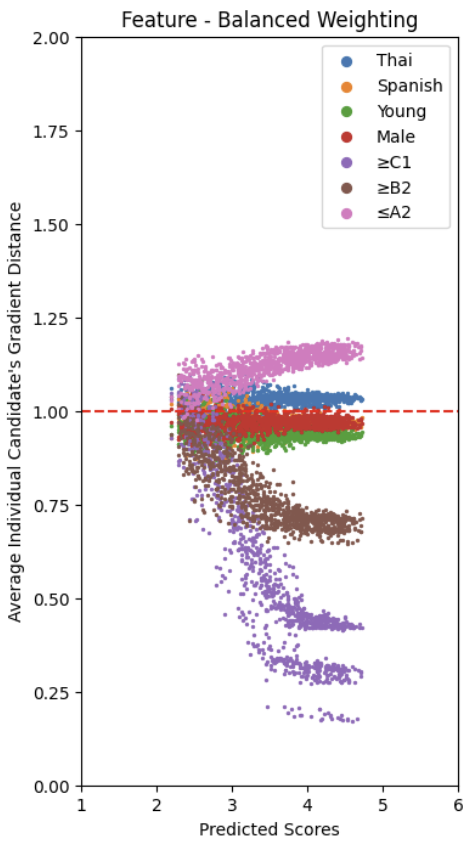
\includegraphics[width=0.48\linewidth]{feature_balanced.png}
        \hfill
        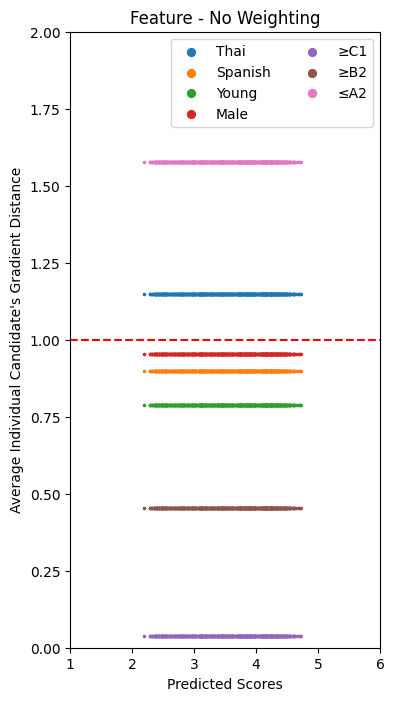
\includegraphics[width=0.48\linewidth]{feature_none.png}
        \caption{$\mathcal{B}^{(ci)}_{gr}$ for feature-based model}
        \label{fig:gradient_distance_feature}
    \end{minipage}
    \hfill
    \begin{minipage}[t]{0.48\textwidth}
        \centering
        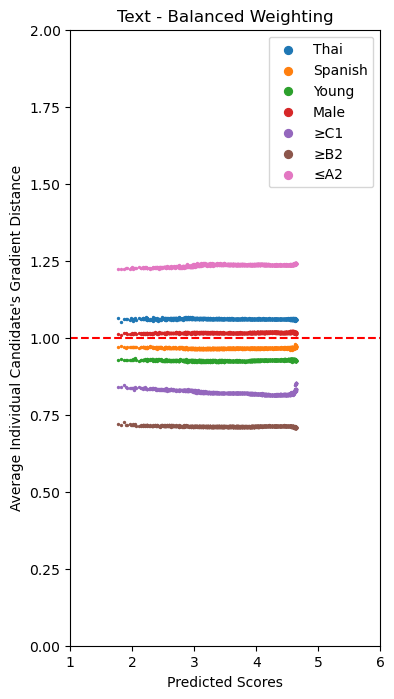
\includegraphics[width=0.48\linewidth]{text_balanced.png}
        \hfill
        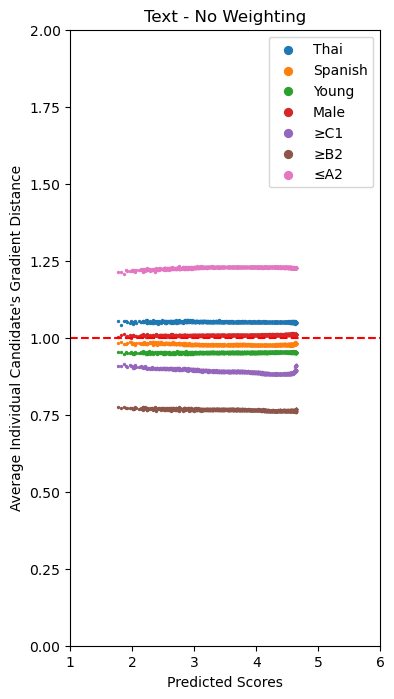
\includegraphics[width=0.48\linewidth]{text_none.png}
        \caption{$\mathcal{B}^{(ci)}_{gr}$ for text-based model}
        \label{fig:gradient_distance_text}
    \end{minipage}
    \hfill
    \begin{minipage}[t]{0.48\textwidth}
        \centering
        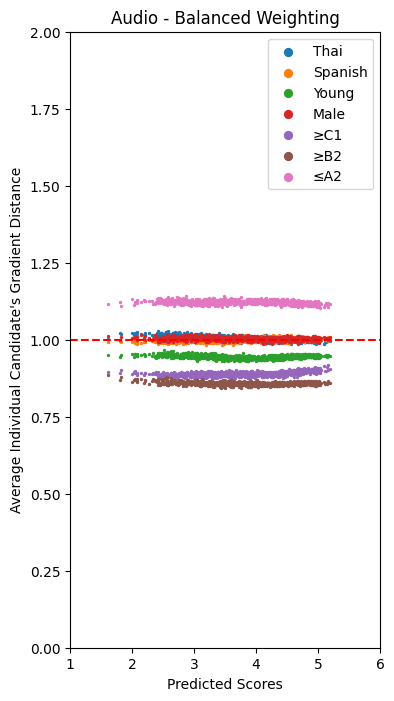
\includegraphics[width=0.48\linewidth]{audio_balanced.png}
        \hfill
        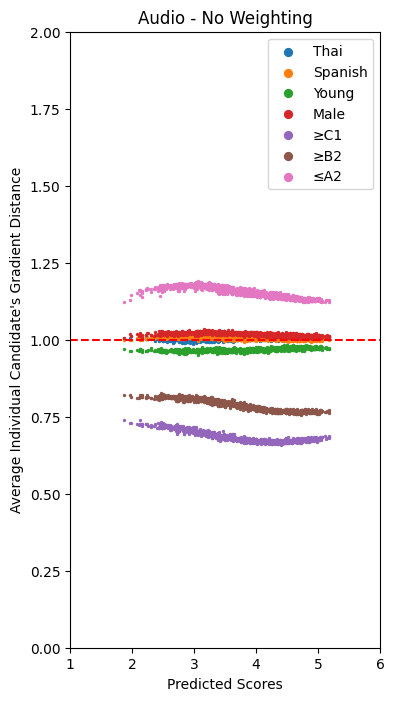
\includegraphics[width=0.48\linewidth]{audio_none.png}
        \caption{$\mathcal{B}^{(ci)}_{gr}$ for audio-based model}
        \label{fig:gradient_distance_audio}
    \end{minipage}
\end{figure}

% \begin{figure}[H]
%     \centering
%     \begin{minipage}[t]{0.32\textwidth}
%         \centering
%         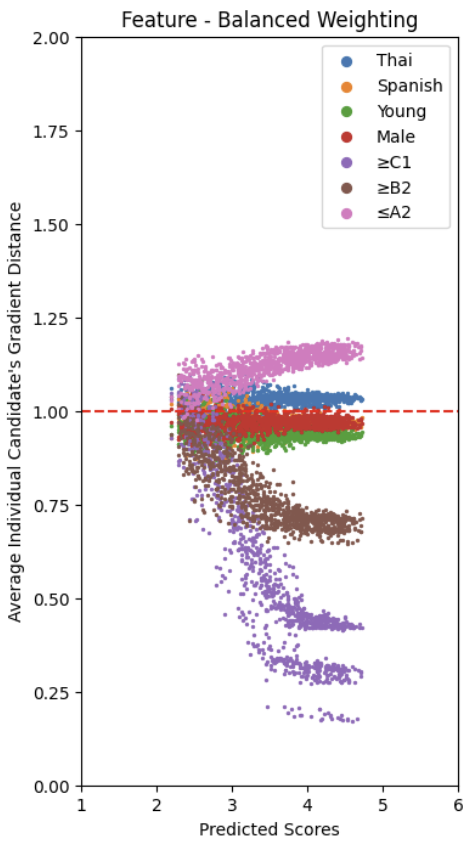
\includegraphics[width=0.48\linewidth]{feature_balanced.png}
%         \hfill
%         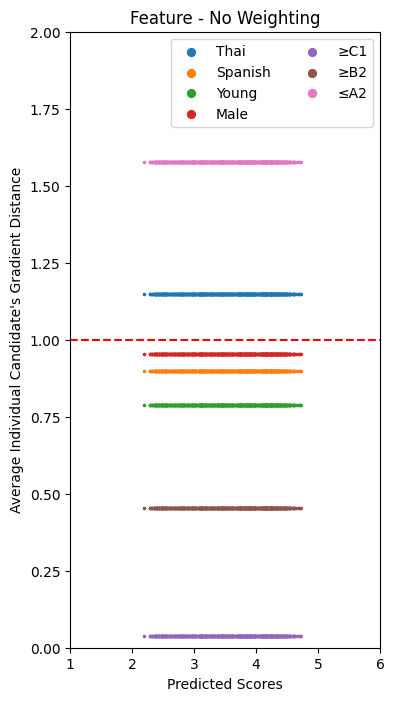
\includegraphics[width=0.48\linewidth]{feature_none.png}
%         \caption{$\mathcal{B}^{(ci)}_{gr}$ for feature-based model}
%         \label{fig:gradient_distance_feature}
%     \end{minipage}
%     \hfill
%     \begin{minipage}[t]{0.32\textwidth}
%         \centering
%         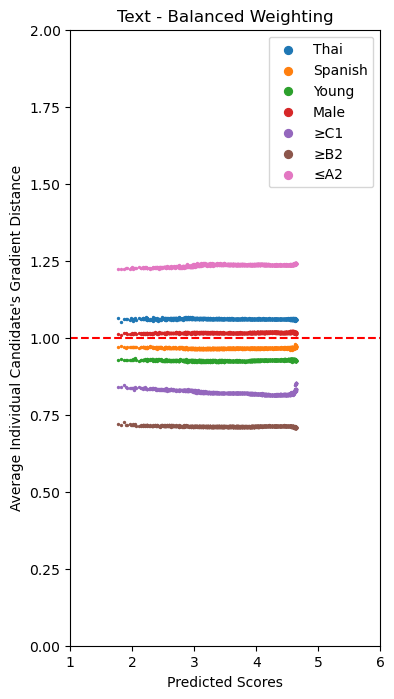
\includegraphics[width=0.48\linewidth]{text_balanced.png}
%         \hfill
%         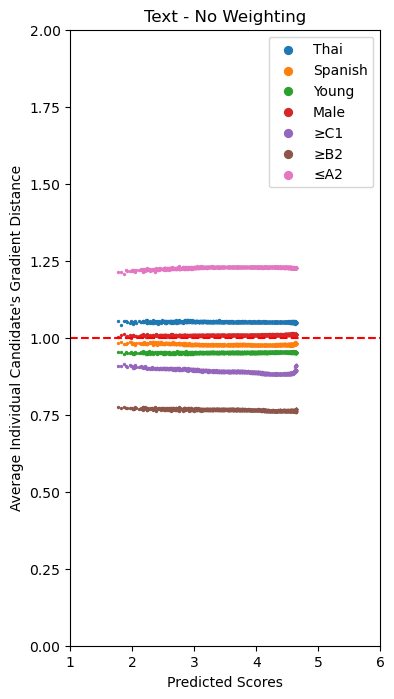
\includegraphics[width=0.48\linewidth]{text_none.png}
%         \caption{$\mathcal{B}^{(ci)}_{gr}$ for text-based model}
%         \label{fig:gradient_distance_text}
%     \end{minipage}
% \end{figure}

% \begin{figure}[H]
%     \centering
%     \resizebox{0.5\textwidth}{!}{
%         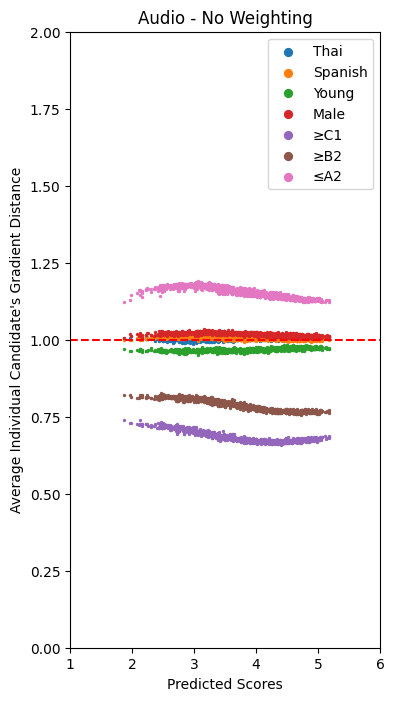
\includegraphics[width=0.48\linewidth]{audio_none.png}
%         \hfill
%         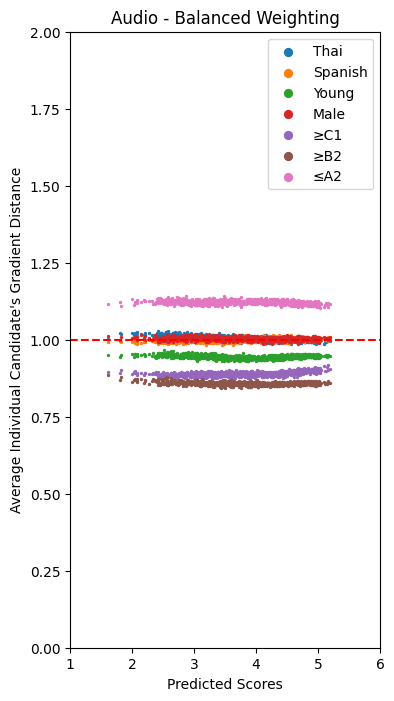
\includegraphics[width=0.48\linewidth]{audio_balanced.png}
%     }
%     \caption{$\mathcal{B}^{(ci)}_{gr}$ for audio-based model}
%     \label{fig:gradient_distance_audio}
% \end{figure}

The results are consistent with the findings from Table \ref{tab:gradient_distance_combined}. The non-grade concepts are close to 1, the `$\leq$ A2' concept is higher than 1, and the `$\geq$ B2' and `$\geq$ C1' concepts are lower than one. The pattern between those from no weighting and balanced weighting is similar. Also, feature-based model has the greatest deviation from 1 for all concepts.

All three graphs consist of a thin, horizontal lines, which shows that the bias measurement of the model is constant across different candidates with different predicted scores. The pattern from feature-based model differs from the pattern in Xizi's paper \cite{feature_bias}, which shows a thicker line with varying $\mathcal{B}^{(ci)}_{gr}$.'s value. However, the pattern extracted from the feature-based model, using the gradient before passing through the activation function, is more similar to the pattern in Xizi's paper (refer to Appendix \ref{app:feature_bias} for the comparison). It is possible that the extract in \cite{feature_bias} are in fact the pre-activation values.

Overall, this section shows that the three models are able to detect the bias from grade-related concepts, with feature-based model being the most sensitive to bias measurement. The CAV accuracy and the use of balanced weighting does not affect the sensitivity to bias measurement. The subsequent results in this chapter are then only presented for CAVs extracted with balanced weighting.

\subsection{Model Biasing} \label{sec:model_biasing}
The results in the previous section (Section \ref{sec:gradient_distance}) show that the three models are able to detect the bias from grade-related concepts. However, for non-grade related concepts, it is unsure whether the models are unbiased towards those concepts, or the CAVs are not able to detect the bias. To further investigate this, models biased towards the non-grade concepts (Thai, Spanish, Young, Male) are trained.

For each biased model, the CAV are used to detected the bias for the concept being biased through computing $\mathcal{B}^{(ci)}_{gr}$. The plot of $\mathcal{B}^{(ci)}_{gr}$ against candidates’ ensemble predicted score of the biased concepts are shown in Figure \ref{fig:grad_spanish_balanced} to \ref{fig:grad_young_balanced}, comparing the results with the original model without biasing.
\begin{figure}[H]
    \centering
    % Spanish
    \begin{subfigure}{0.32\textwidth}
        \centering
        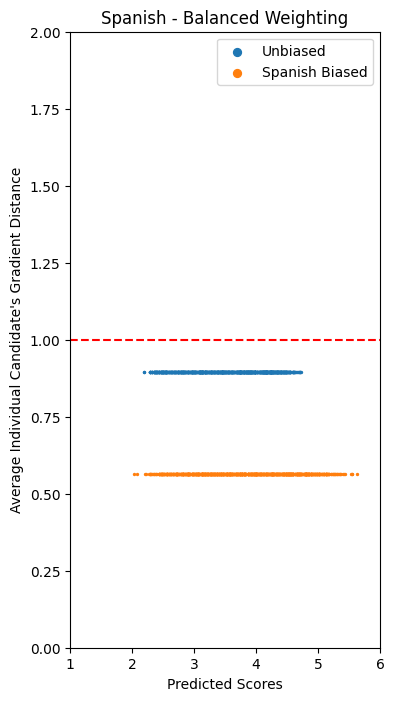
\includegraphics[width=0.7\linewidth]{Feature/spanish_part1_input_layer_balanced.png}
    \end{subfigure}
    \hfill
    \begin{subfigure}{0.32\textwidth}
        \centering
        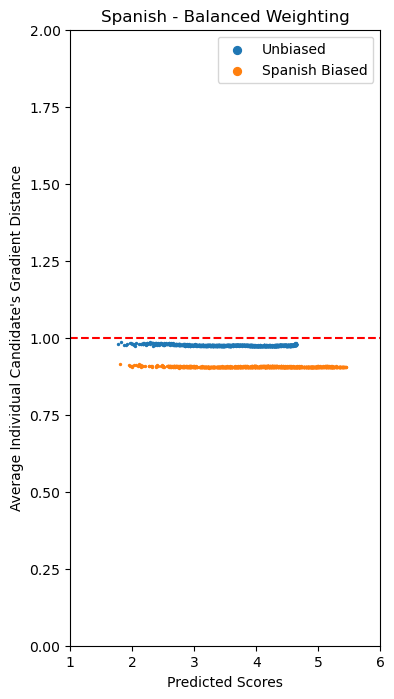
\includegraphics[width=0.7\linewidth]{Text/spanish_part1_layer1_balanced.png}
    \end{subfigure}
    \hfill
    \begin{subfigure}{0.32\textwidth}
        \centering
        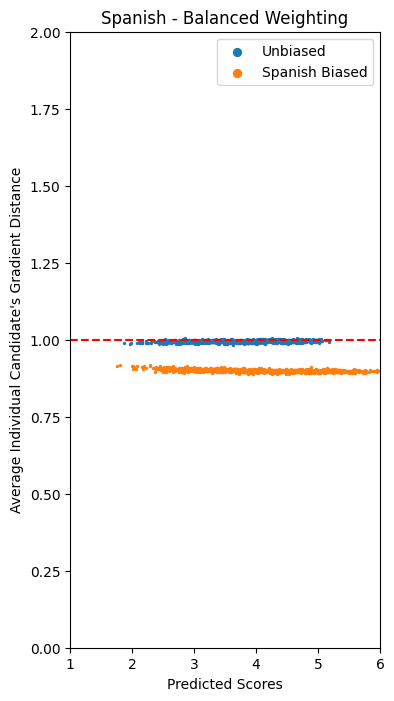
\includegraphics[width=0.7\linewidth]{Audio/spanish_part1_dense_balanced.png}
    \end{subfigure}
    \caption{$\mathcal{B}^{(ci)}_{gr}$ for Spanish concept for feature, text and audio-based model, left to right}
    \label{fig:grad_spanish_balanced}
\end{figure}

\begin{figure}[H]
    \centering
    % Thai
    \begin{subfigure}{0.32\textwidth}
        \centering
        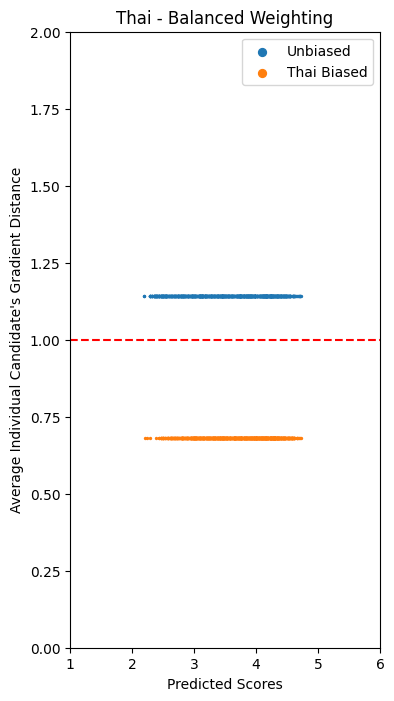
\includegraphics[width=0.7\linewidth]{Feature/thai_part1_input_layer_balanced.png}
    \end{subfigure}
    \hfill
    \begin{subfigure}{0.32\textwidth}
        \centering
        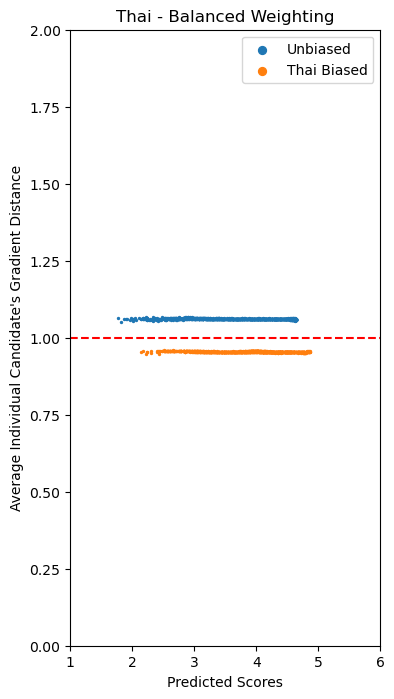
\includegraphics[width=0.7\linewidth]{Text/thai_part1_layer1_balanced.png}
    \end{subfigure}
    \hfill
    \begin{subfigure}{0.32\textwidth}
        \centering
        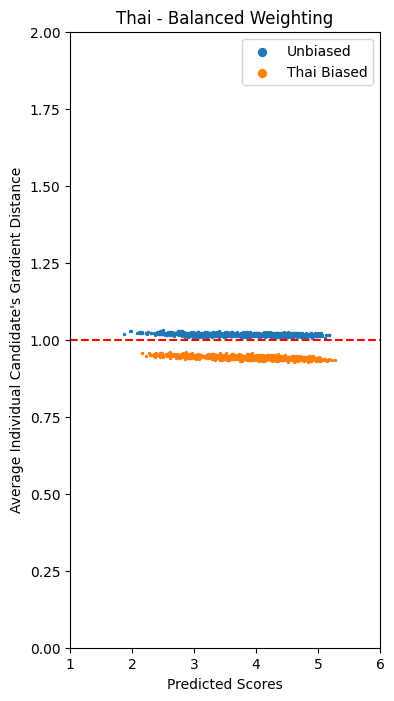
\includegraphics[width=0.7\linewidth]{Audio/thai_part1_dense_balanced.png}
    \end{subfigure}
    \caption{$\mathcal{B}^{(ci)}_{gr}$ for Thai concept for feature, text and audio-based model, left to right}
    \label{fig:grad_thai_balanced}
\end{figure}

\begin{figure}[H]
    \centering
    % Male
    \begin{subfigure}{0.32\textwidth}
        \centering
        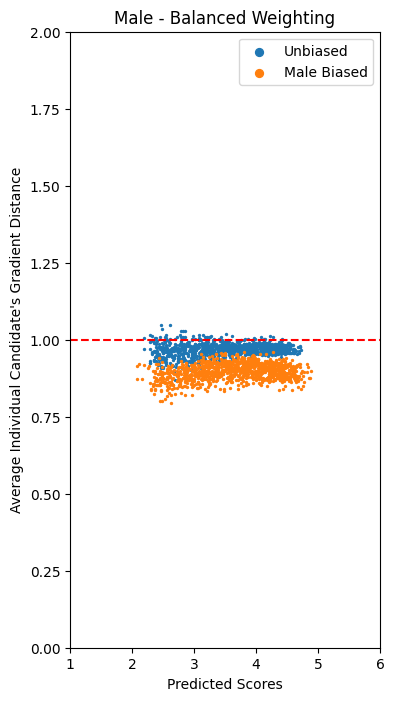
\includegraphics[width=0.7\linewidth]{Feature/male_part1_input_layer_balanced.png}
    \end{subfigure}
    \hfill
    \begin{subfigure}{0.32\textwidth}
        \centering
        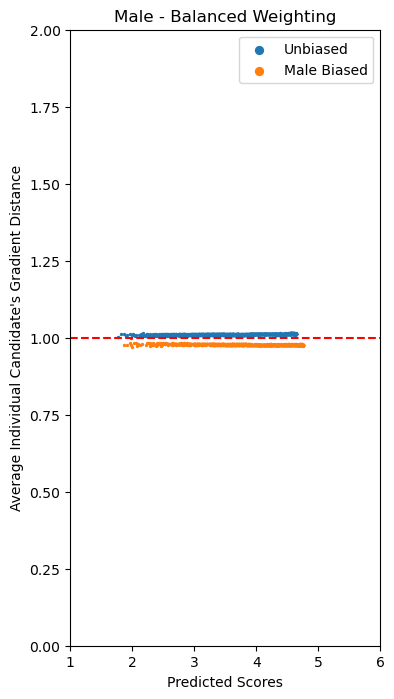
\includegraphics[width=0.7\linewidth]{Text/male_part1_layer1_balanced.png}
    \end{subfigure}
    \hfill
    \begin{subfigure}{0.32\textwidth}
        \centering
        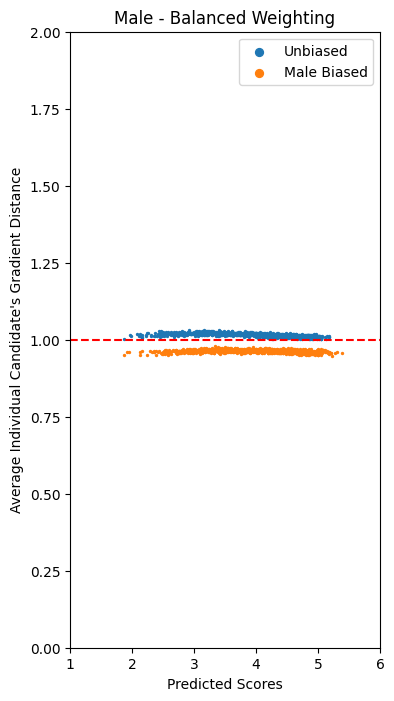
\includegraphics[width=0.7\linewidth]{Audio/male_part1_dense_balanced.png}
    \end{subfigure}
    \caption{$\mathcal{B}^{(ci)}_{gr}$ for Male concept for feature, text and audio-based model, left to right}
    \label{fig:grad_male_balanced}
\end{figure}

\begin{figure}[H]
    \centering
    % Young
    \begin{subfigure}{0.32\textwidth}
        \centering
        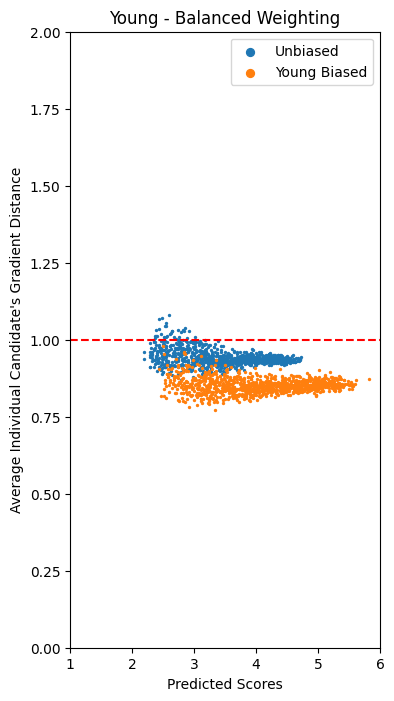
\includegraphics[width=0.7\linewidth]{Feature/young_part1_input_layer_balanced.png}
    \end{subfigure}
    \hfill
    \begin{subfigure}{0.32\textwidth}
        \centering
        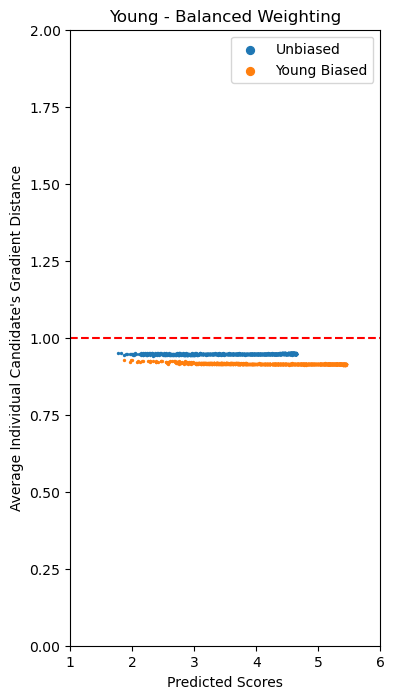
\includegraphics[width=0.7\linewidth]{Text/young_part1_layer1_balanced.png}
    \end{subfigure}
    \hfill
    \begin{subfigure}{0.32\textwidth}
        \centering
        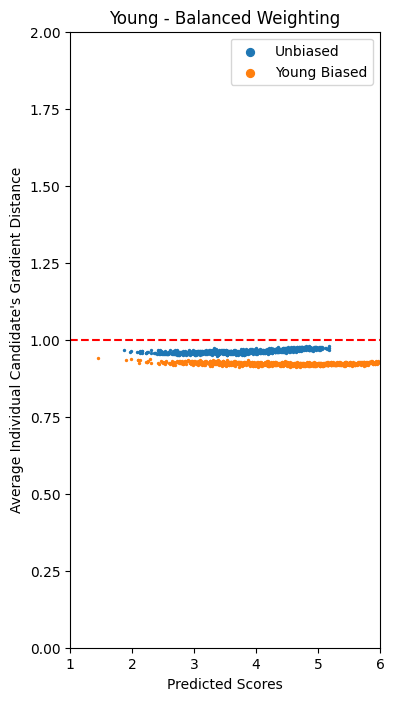
\includegraphics[width=0.7\linewidth]{Audio/young_part1_dense_balanced.png}
    \end{subfigure}
    \caption{$\mathcal{B}^{(ci)}_{gr}$ for Young concept for feature, text and audio-based model, left to right}
    \label{fig:grad_young_balanced}
\end{figure}

% \begin{figure}[H]
%     \centering
%     % First pair
%     \begin{minipage}[t]{0.48\textwidth}
%         \centering
%         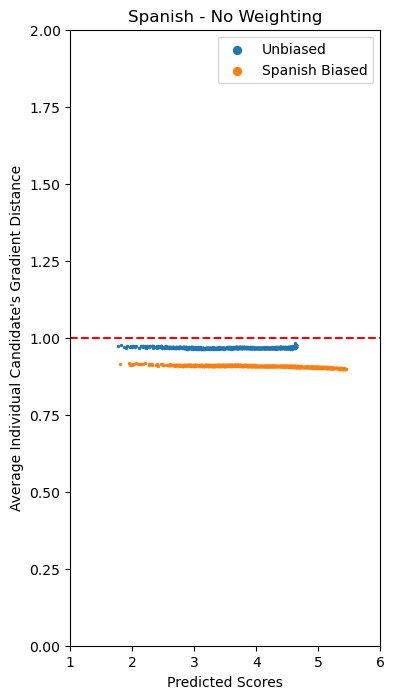
\includegraphics[width=0.32\linewidth]{Text/spanish_part1_layer1.png}
%         \hfill
%         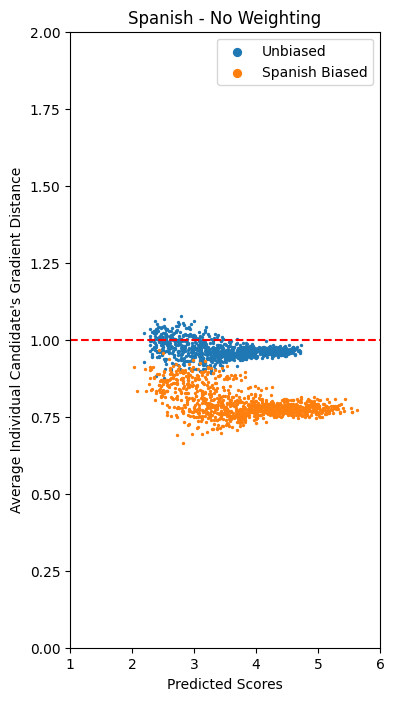
\includegraphics[width=0.32\linewidth]{Feature/spanish_part1_input_layer.png}
%         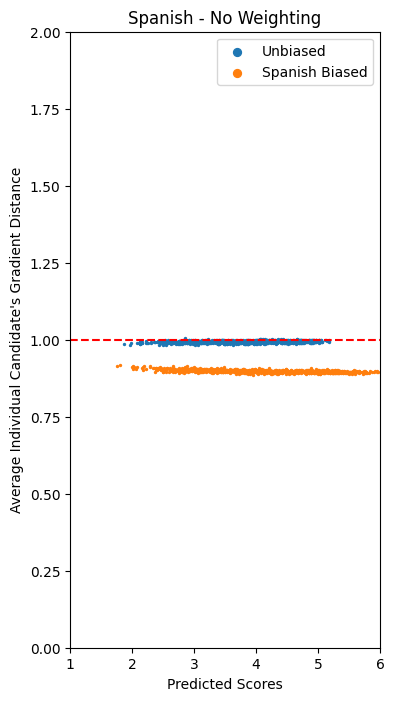
\includegraphics[width=0.32\linewidth]{Audio/spanish_part1_dense.png}
%         \caption{$\mathcal{B}^{(ci)}_{gr}$ for spanish concept across text, feature and audio-based model (left to right), no weighting}
%         \label{fig:grad_spanish}
%     \end{minipage}
%     \hfill
%     % Second pair
%     \begin{minipage}[t]{0.48\textwidth}
%         \centering
%         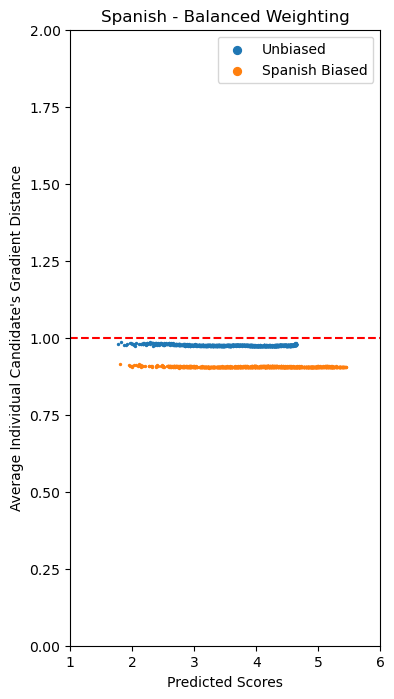
\includegraphics[width=0.32\linewidth]{Text/spanish_part1_layer1_balanced.png}
%         \hfill
%         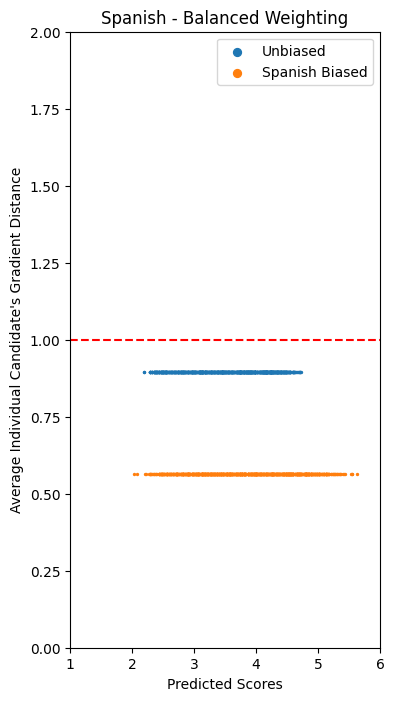
\includegraphics[width=0.32\linewidth]{Feature/spanish_part1_input_layer_balanced.png}
%         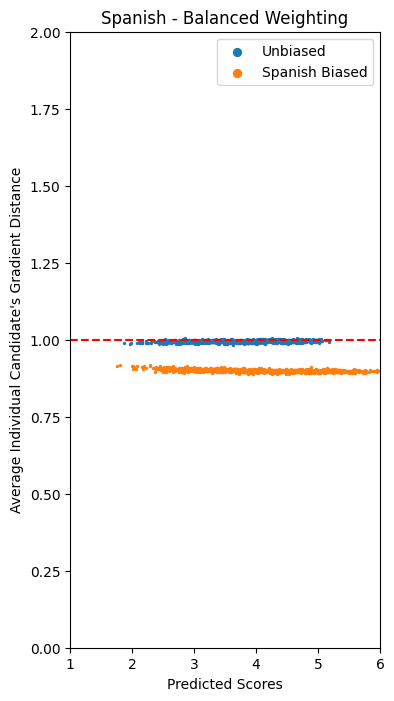
\includegraphics[width=0.32\linewidth]{Audio/spanish_part1_dense_balanced.png}
%         \caption{$\mathcal{B}^{(ci)}_{gr}$ for spanish concept across text, feature and audio-based model (left to right), balanced weighting}
%         \label{fig:grad_spanish_balanced}
%     \end{minipage}
% \end{figure}

% \begin{figure}[H]
%     \centering
%     % First pair
%     \begin{minipage}[t]{0.48\textwidth}
%         \centering
%         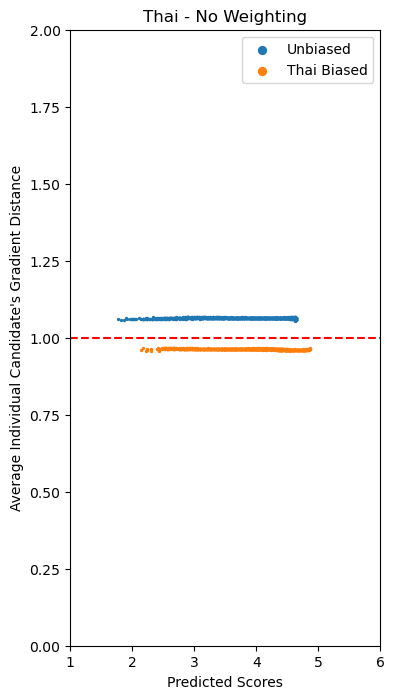
\includegraphics[width=0.32\linewidth]{Text/thai_part1_layer1.png}
%         \hfill
%         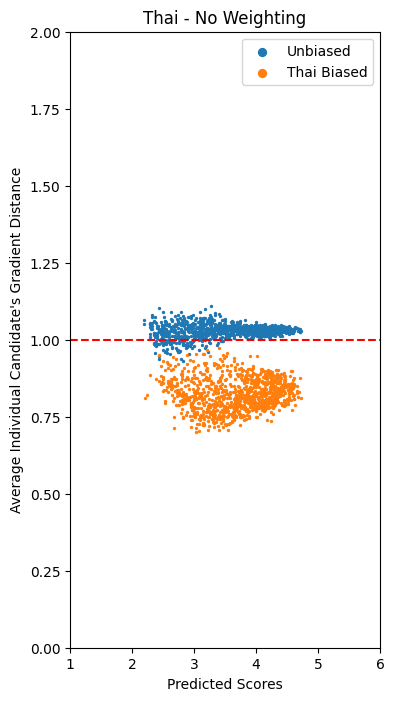
\includegraphics[width=0.32\linewidth]{Feature/thai_part1_input_layer.png}
%         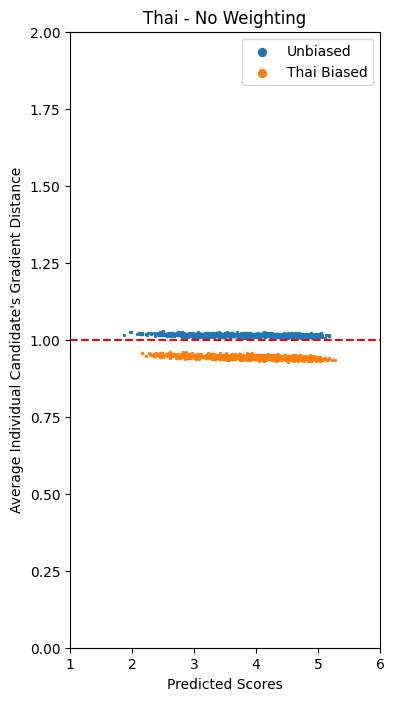
\includegraphics[width=0.32\linewidth]{Audio/thai_part1_dense.png}
%         \caption{$\mathcal{B}^{(ci)}_{gr}$ for thai concept across text, feature and audio-based model (left to right), no weighting}
%         \label{fig:grad_thai}
%     \end{minipage}
%     \hfill
%     % Second pair
%     \begin{minipage}[t]{0.48\textwidth}
%         \centering
%         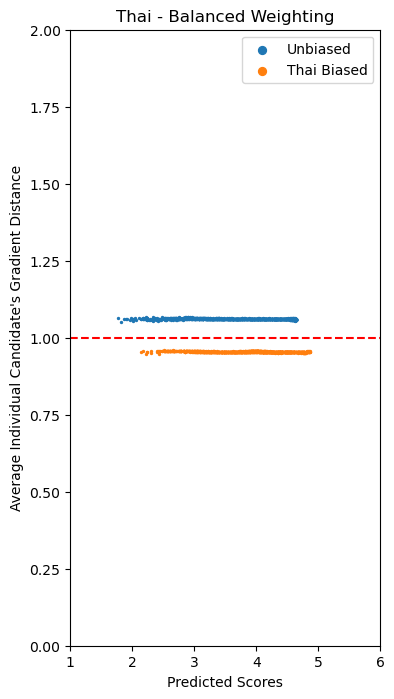
\includegraphics[width=0.32\linewidth]{Text/thai_part1_layer1_balanced.png}
%         \hfill
%         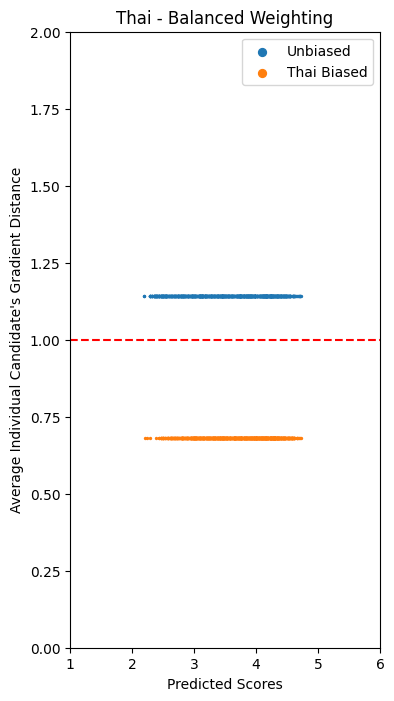
\includegraphics[width=0.32\linewidth]{Feature/thai_part1_input_layer_balanced.png}
%         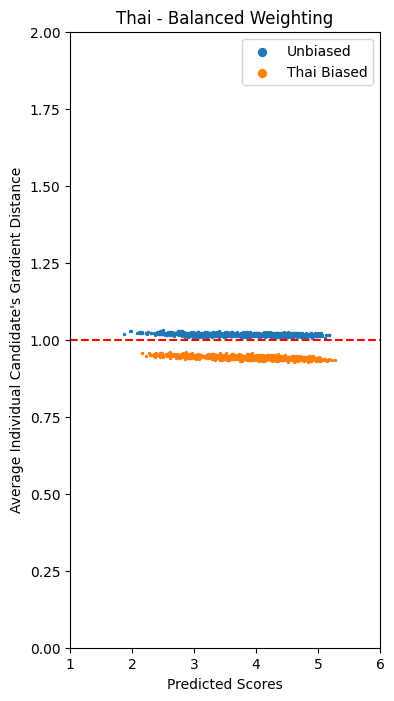
\includegraphics[width=0.32\linewidth]{Audio/thai_part1_dense_balanced.png}
%         \caption{$\mathcal{B}^{(ci)}_{gr}$ for thai concept across text, feature and audio-based model (left to right), balanced weighting}
%         \label{fig:grad_thai_balanced}
%     \end{minipage}
% \end{figure}

% \begin{figure}[H]
%     \centering
%     % First pair
%     \begin{minipage}[t]{0.48\textwidth}
%         \centering
%         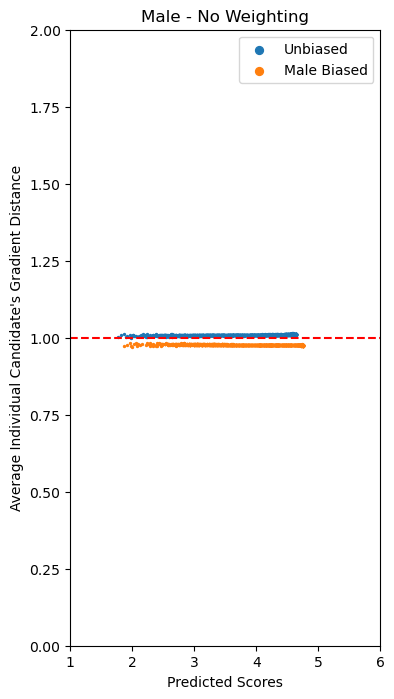
\includegraphics[width=0.32\linewidth]{Text/male_part1_layer1.png}
%         \hfill
%         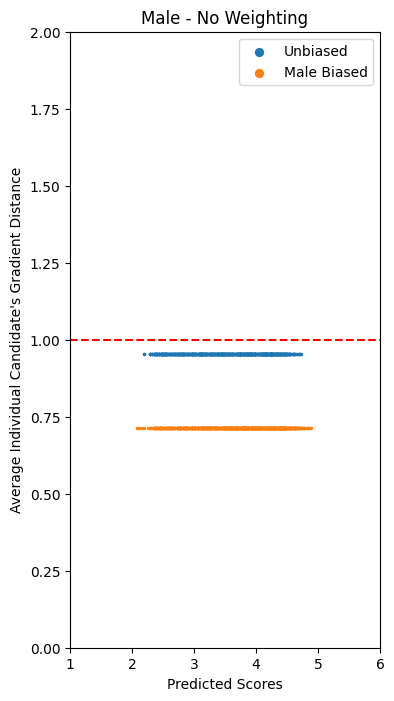
\includegraphics[width=0.32\linewidth]{Feature/male_part1_input_layer.png}
%         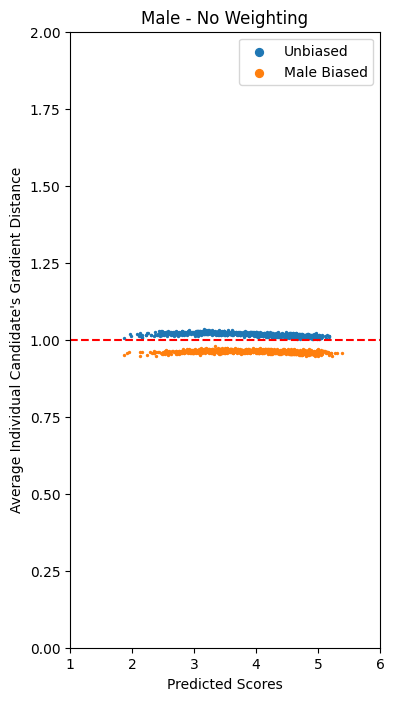
\includegraphics[width=0.32\linewidth]{Audio/male_part1_dense.png}
%         \caption{$\mathcal{B}^{(ci)}_{gr}$ for male concept across text, feature and audio-based model (left to right), no weighting}
%         \label{fig:grad_male}
%     \end{minipage}
%     \hfill
%     % Second pair
%     \begin{minipage}[t]{0.48\textwidth}
%         \centering
%         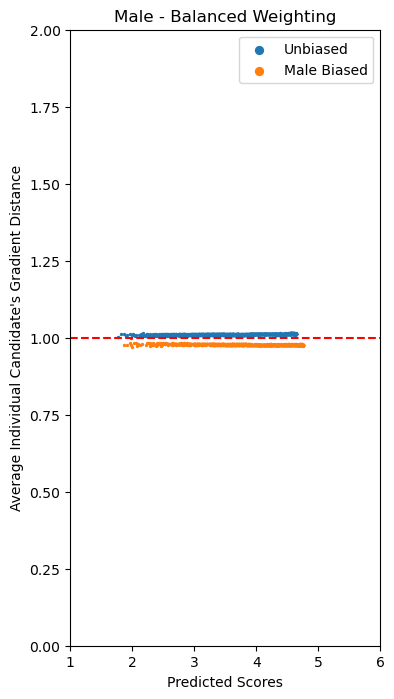
\includegraphics[width=0.32\linewidth]{Text/male_part1_layer1_balanced.png}
%         \hfill
%         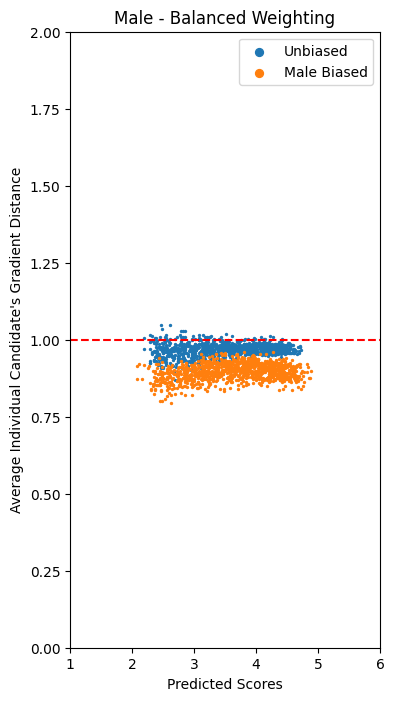
\includegraphics[width=0.32\linewidth]{Feature/male_part1_input_layer_balanced.png}
%         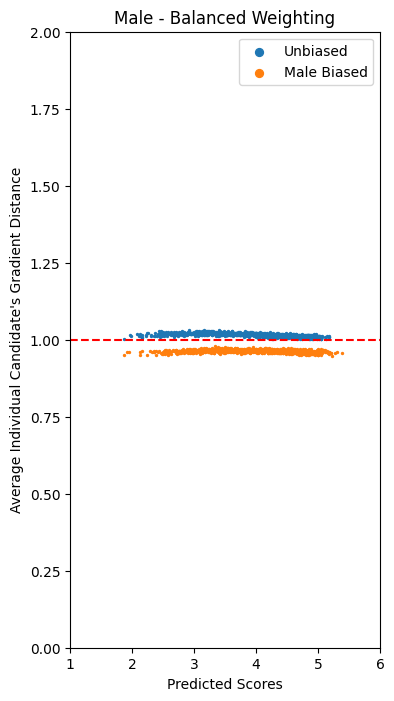
\includegraphics[width=0.32\linewidth]{Audio/male_part1_dense_balanced.png}
%         \caption{$\mathcal{B}^{(ci)}_{gr}$ for male concept across text, feature and audio-based model (left to right), balanced weighting}
%         \label{fig:grad_male_balanced}
%     \end{minipage}
% \end{figure}

% \begin{figure}[H]
%     \centering
%     % First pair
%     \begin{minipage}[t]{0.48\textwidth}
%         \centering
%         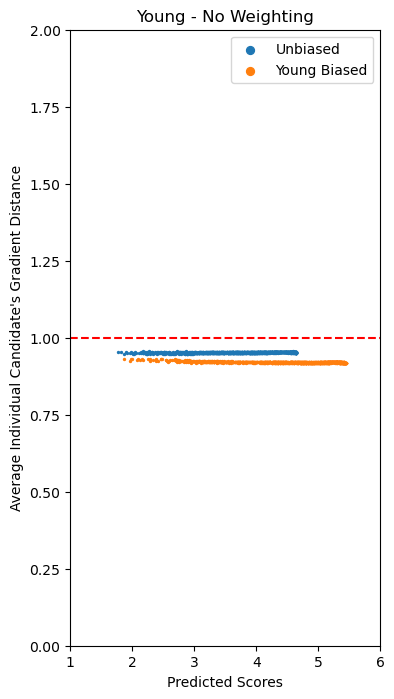
\includegraphics[width=0.32\linewidth]{Text/young_part1_layer1.png}
%         \hfill
%         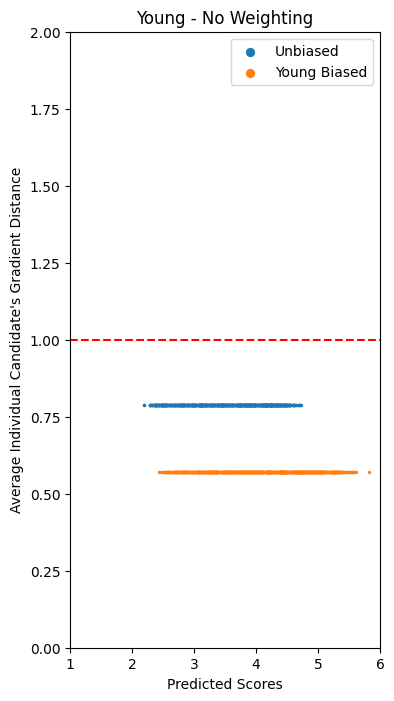
\includegraphics[width=0.32\linewidth]{Feature/young_part1_input_layer.png}
%         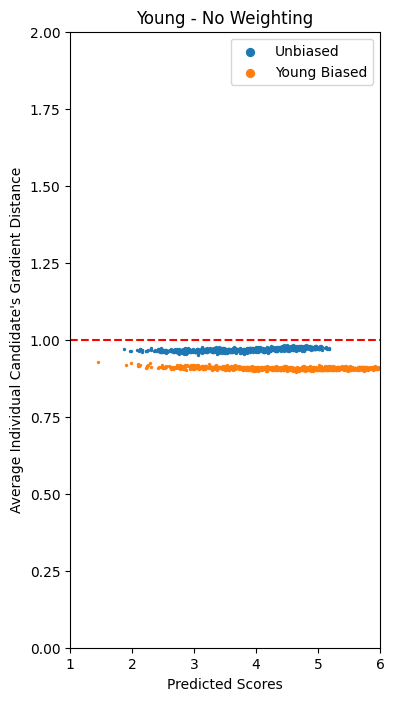
\includegraphics[width=0.32\linewidth]{Audio/young_part1_dense.png}
%         \caption{$\mathcal{B}^{(ci)}_{gr}$ for young concept across text, feature and audio-based model (left to right), no weighting}
%         \label{fig:grad_young}
%     \end{minipage}
%     \hfill
%     % Second pair
%     \begin{minipage}[t]{0.48\textwidth}
%         \centering
%         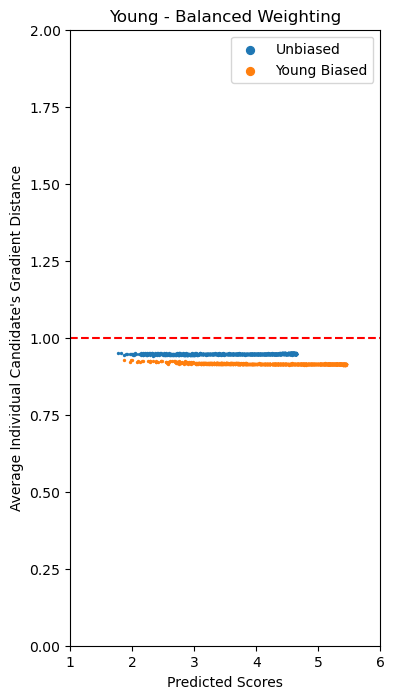
\includegraphics[width=0.32\linewidth]{Text/young_part1_layer1_balanced.png}
%         \hfill
%         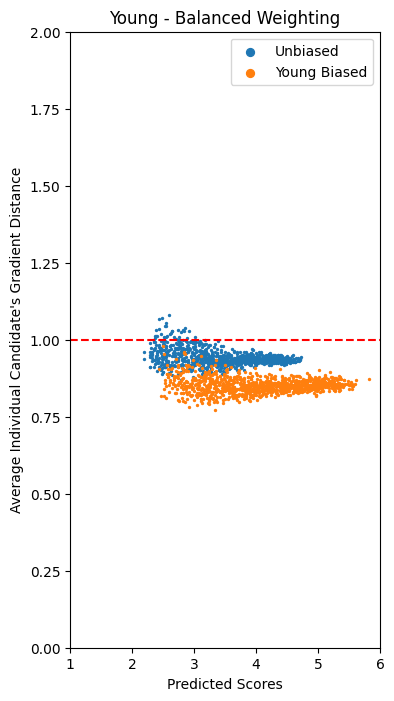
\includegraphics[width=0.32\linewidth]{Feature/young_part1_input_layer_balanced.png}
%         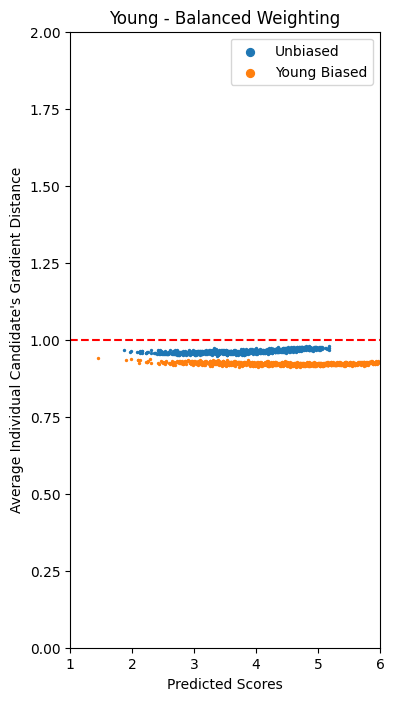
\includegraphics[width=0.32\linewidth]{Audio/young_part1_dense_balanced.png}
%         \caption{$\mathcal{B}^{(ci)}_{gr}$ for young concept across text, feature and audio-based model (left to right), balanced weighting}
%         \label{fig:grad_young_balanced}
%     \end{minipage}
% \end{figure}

% \begin{figure}[H]
%     \centering
%     \begin{minipage}{0.23\textwidth}
%         \begin{figure}[H]
%             \centering
%             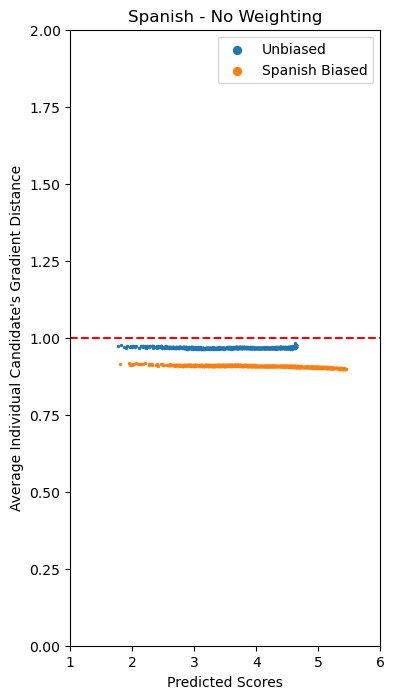
\includegraphics[width=0.9\textwidth]{Text/spanish_part1_layer1.png}
%         \end{figure}
%     \end{minipage}
%     \begin{minipage}{0.23\textwidth}
%         \begin{figure}[H]
%             \centering
%             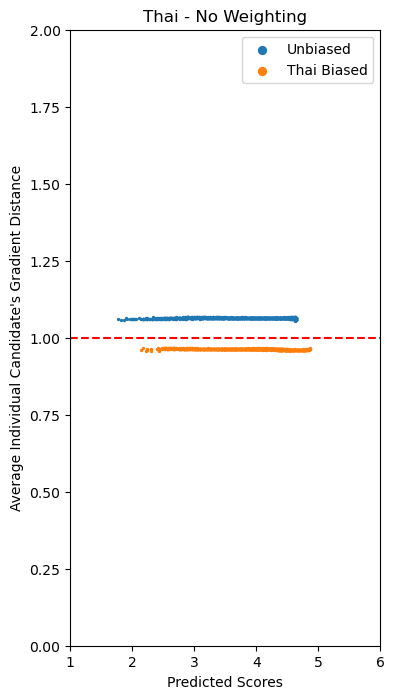
\includegraphics[width=0.9\textwidth]{Text/thai_part1_layer1.png}
%         \end{figure}
%     \end{minipage}
%     \begin{minipage}{0.23\textwidth}
%         \begin{figure}[H]
%             \centering
%             \includegraphics[width=0.9\textwidth]{Text/male_part1_layer1.png}
%         \end{figure}
%     \end{minipage}
%     \begin{minipage}{0.23\textwidth}
%         \begin{figure}[H]
%             \centering
%             \includegraphics[width=0.9\textwidth]{Text/young_part1_layer1.png}
%         \end{figure}
%     \end{minipage}
%     \caption{$\mathcal{B}_{gr}^{(ci)}$ for text-based model with no weighting}
%     \label{fig:grad_text}
% \end{figure}

% \begin{figure}[H]
%     \centering
%     \begin{minipage}{0.23\textwidth}
%         \begin{figure}[H]
%             \centering
%             \includegraphics[width=0.9\textwidth]{Text/spanish_part1_layer1_balanced.png}
%         \end{figure}
%     \end{minipage}
%     \begin{minipage}{0.23\textwidth}
%         \begin{figure}[H]
%             \centering
%             \includegraphics[width=0.9\textwidth]{Text/thai_part1_layer1_balanced.png}
%         \end{figure}
%     \end{minipage}
%     \begin{minipage}{0.23\textwidth}
%         \begin{figure}[H]
%             \centering
%             \includegraphics[width=0.9\textwidth]{Text/male_part1_layer1_balanced.png}
%         \end{figure}
%     \end{minipage}
%     \begin{minipage}{0.23\textwidth}
%         \begin{figure}[H]
%             \centering
%             \includegraphics[width=0.9\textwidth]{Text/young_part1_layer1_balanced.png}
%         \end{figure}
%     \end{minipage}
%     \caption{$\mathcal{B}_{gr}^{(ci)}$ for text-based model with balanced weighting}
%     \label{fig:grad_text_balanced}
% \end{figure}

% \begin{figure}[H]
%     \centering
%     \begin{minipage}{0.23\textwidth}
%         \begin{figure}[H]
%             \centering
%             \includegraphics[width=0.9\textwidth]{Feature/spanish_part1_input_layer.png}
%         \end{figure}
%     \end{minipage}
%     \begin{minipage}{0.23\textwidth}
%         \begin{figure}[H]
%             \centering
%             \includegraphics[width=0.9\textwidth]{Feature/thai_part1_input_layer.png}
%         \end{figure}
%     \end{minipage}
%     \begin{minipage}{0.23\textwidth}
%         \begin{figure}[H]
%             \centering
%             \includegraphics[width=0.9\textwidth]{Feature/male_part1_input_layer.png}
%         \end{figure}
%     \end{minipage}
%     \begin{minipage}{0.23\textwidth}
%         \begin{figure}[H]
%             \centering
%             \includegraphics[width=0.9\textwidth]{Feature/young_part1_input_layer.png}
%         \end{figure}
%     \end{minipage}
%     \caption{$\mathcal{B}_{gr}^{(ci)}$ for feature-based model with no weighting}
%     \label{fig:grad_feature}
% \end{figure}

% \begin{figure}[H]
%     \centering
%     \begin{minipage}{0.23\textwidth}
%         \begin{figure}[H]
%             \centering
%             \includegraphics[width=0.9\textwidth]{Feature/spanish_part1_input_layer_balanced.png}
%         \end{figure}
%     \end{minipage}
%     \begin{minipage}{0.23\textwidth}
%         \begin{figure}[H]
%             \centering
%             \includegraphics[width=0.9\textwidth]{Feature/thai_part1_input_layer_balanced.png}
%         \end{figure}
%     \end{minipage}
%     \begin{minipage}{0.23\textwidth}
%         \begin{figure}[H]
%             \centering
%             \includegraphics[width=0.9\textwidth]{Feature/male_part1_input_layer_balanced.png}
%         \end{figure}
%     \end{minipage}
%     \begin{minipage}{0.23\textwidth}
%         \begin{figure}[H]
%             \centering
%             \includegraphics[width=0.9\textwidth]{Feature/young_part1_input_layer_balanced.png}
%         \end{figure}
%     \end{minipage}
%     \caption{$\mathcal{B}_{gr}^{(ci)}$ for feature-based model with balanced weighting}
%     \label{fig:grad_feature_balanced}
% \end{figure}

% \begin{figure}[H]
%     \centering
%     \begin{minipage}{0.23\textwidth}
%         \begin{figure}[H]
%             \centering
%             \includegraphics[width=0.9\textwidth]{Audio/spanish_part1_dense.png}
%         \end{figure}
%     \end{minipage}
%     \begin{minipage}{0.23\textwidth}
%         \begin{figure}[H]
%             \centering
%             \includegraphics[width=0.9\textwidth]{Audio/thai_part1_dense.png}
%         \end{figure}
%     \end{minipage}
%     \begin{minipage}{0.23\textwidth}
%         \begin{figure}[H]
%             \centering
%             \includegraphics[width=0.9\textwidth]{Audio/male_part1_dense.png}
%         \end{figure}
%     \end{minipage}
%     \begin{minipage}{0.23\textwidth}
%         \begin{figure}[H]
%             \centering
%             \includegraphics[width=0.9\textwidth]{Audio/young_part1_dense.png}
%         \end{figure}
%     \end{minipage}
%     \caption{$\mathcal{B}_{gr}^{(ci)}$ for text-based model with no weighting}
%     \label{fig:grad_audio}
% \end{figure}

% \begin{figure}[H]
%     \centering
%     \begin{minipage}{0.23\textwidth}
%         \begin{figure}[H]
%             \centering
%             \includegraphics[width=0.9\textwidth]{Audio/spanish_part1_dense_balanced.png}
%         \end{figure}
%     \end{minipage}
%     \begin{minipage}{0.23\textwidth}
%         \begin{figure}[H]
%             \centering
%             \includegraphics[width=0.9\textwidth]{Audio/thai_part1_dense_balanced.png}
%         \end{figure}
%     \end{minipage}
%     \begin{minipage}{0.23\textwidth}
%         \begin{figure}[H]
%             \centering
%             \includegraphics[width=0.9\textwidth]{Audio/male_part1_dense_balanced.png}
%         \end{figure}
%     \end{minipage}
%     \begin{minipage}{0.23\textwidth}
%         \begin{figure}[H]
%             \centering
%             \includegraphics[width=0.9\textwidth]{Audio/young_part1_dense_balanced.png}
%         \end{figure}
%     \end{minipage}
%     \caption{$\mathcal{B}_{gr}^{(ci)}$ for audio-based model with balanced weighting}
%     \label{fig:grad_audio_balanced}
% \end{figure}

The results from model biasing is aligned with the results found in Section \ref{sec:gradient_distance}. As before, it is observed that the pattern of $\mathcal{B}^{(ci)}_{gr}$ between graphs without weighting and balanced weighting is similar. This indicates that either method is able to detect the bias equally for the concepts.

In addition, aligning with previous results, the change in $\mathcal{B}^{(ci)}_{gr}$ for the feature-based model is more significant than the text-based and audio-based models, with the gap of $\mathcal{B}^{(ci)}_{gr}$ between the original and bias models being the widest. This verifies that the feature-based model is more sensitive to the bias presence, such that the CAVs are able to detect the bias presence better.

It is found that CAV are more sensitive to L1-related biases. From the figures, the change in $\mathcal{B}^{(ci)}_{gr}$ within L1-related concepts (Thai, Spanish), particularly Spanish, is more significant compared to other concepts across all three models. For non-L1 concepts (Male, Young), the change is negligible in text and audio-based models, hence the CAVs are actually unable to detect biases presence for those concepts. It is interesting to observe that the text-based model has its $\mathcal{B}^{(ci)}_{gr}$ deviating more from 1 for the original model than the biased version, which might indicate the initial model has slight bias towards Thai speaker. Regardless, the results reflect that CAVs are better in detecting bias presence for L1-related concepts than non-L1 concepts in these models.

The result further supports the lack of correlation between CAV accuracy and sensitivity to bias presence. From Table \ref{tab:CAV_accuracy_combined}, the CAV accuracy for audio-based model is the highest, yet it is much less sensitive than feature-based model in detecting bias presence. In contrast, L1-related (Thai, Spanish) CAV has a higher CAV accuracy, and the result does show that CAVs are generally more sensitive to biases in L1-related concepts.

Overall, this shows that CAV can best detect bias towards L1-concepts, particularly Spanish L1-speaker in feature-based models compared to other concepts and models. It is unable to detect non-L1 related biases in text and audio-based models. It also supports the finding in Section \ref{sec:gradient_distance} that CAV accuracy and the use of balanced weighting does not affect the sensitivity to bias measurement.

\section{Factor Isolation} \label{sec:factor_isolation}
This section presents the result of the experiments performed on the modified models to isolate the effect of different factors on the bias measurement. The previous section (Section \ref{sec:bias_detection}) shows that plots of $\mathcal{B}^{(ci)}_{gr}$ against ensemble score for feature-based model spans wider than text and audio based model. The models differ in network architecture, model type, activation function, and input type, which are all possible factors that could influence $\mathcal{B}^{(ci)}_{gr}$'s pattern. Hence, they are evaluated to uncover the factors affecting the pattern. The results are compared with the original models to see the changes in pattern. All the CAVs are extracted with balanced weighting.

\subsection{Network Architecture} \label{sec:network_architecture}
The first experiment changes the network of the feature-based model to the network from the text-based model (Figure \ref{fig:bert_like}). The changes including the node and layer number, and dropout rate, with the feature vector retained as input, and activation function kept as LReLU. This is to see if the architecture of the network affects the bias measurement.

The accuracy of the modified feature-based model is compared with the original feature-based model, as shown in Table \ref{tab:model_accuracy_bert_like}. The coefficients for the linear calibration of both models are presented in Table \ref{tab:linear_regression_coefficients_bert_like} as a reference. The results show that the modified model is decent and even perform slightly better than the original feature-based model, indicating that the architecture change does not affect the model performance significantly, hence reliable for CAV extraction.

\begin{table}[H]
    \centering
    \begin{tabular}{|lc|c|c|c|c|}
        \hline
        \multicolumn{2}{|l|}{\textbf{}}                                         & \textbf{RMSE}         & \textbf{PCC} & \textbf{\textless 0.5} & \textbf{\textless 1}        \\ \hline
        \multicolumn{1}{|l|}{\multirow{2}{*}{\textbf{Original Architecture}}}   & \textbf{Uncalibrated} & 0.694        & 0.821                  & 55.3                 & 83.4 \\ \cline{2-6}
        \multicolumn{1}{|l|}{}                                                  & \textbf{Calibrated}   & 0.638        & 0.821                  & 56.6                 & 87.9 \\ \hline
        \multicolumn{1}{|l|}{\multirow{2}{*}{\textbf{Text-based Architecture}}} & \textbf{Uncalibrated} & 0.670        & 0.826                  & 57.2                 & 86.6 \\ \cline{2-6}
        \multicolumn{1}{|l|}{}                                                  & \textbf{Calibrated}   & 0.631        & 0.826                  & 59.5                 & 88.5 \\ \hline
    \end{tabular}
    \caption{Model accuracy for the feature-based model with the original and text-based network architecture, both calibrated and uncalibrated.}
    \label{tab:model_accuracy_bert_like}
\end{table}


\begin{table}[H]
    \centering
    \begin{tabular}{|l|c|c|}
        \hline
        \textbf{}                        & \textbf{Slope (m)} & \textbf{Intercept (c)} \\ \hline
        \textbf{Original Architecture}   & 1.42               & -1.45                  \\ \hline
        \textbf{Text-based Architecture} & 1.32               & -1.16                  \\ \hline
    \end{tabular}
    \caption{Linear calibration coefficients for the feature-based model with the original and text-based network architecture}
    \label{tab:linear_regression_coefficients_bert_like}
\end{table}

The accuracy of the CAVs extracted from the modified feature-based model is shown in Table \ref{tab:CAV_accuracy_bert_like}. The results show that the CAVs from the modified model are able to differentiate the positive and negative targets with reasonable accuracy, and in fact slightly better than the original feature-based model. Hence, it could be used to measure bias reliably.

\begin{table}[H]
    \centering
    \begin{tabular}{|c|cc|cc|}
        \hline
        \multirow{2}{*}{\textbf{Concept}}
                  & \multicolumn{2}{c|}{\shortstack{\textbf{Original}                                        \\ \textbf{Architecture}}}
                  & \multicolumn{2}{c|}{\shortstack{\textbf{Text-based}                                      \\ \textbf{Architecture}}} \\ \cline{2-5}
                  & \multicolumn{1}{c|}{\textbf{+ve}}                   & \textbf{-ve}
                  & \multicolumn{1}{c|}{\textbf{+ve}}                   & \textbf{-ve}                       \\ \hline

        $\geq$ C1 & \multicolumn{1}{c|}{$94.0_{\pm 0.5}$}               & $76.9_{\pm 1.8}$
                  & \multicolumn{1}{c|}{$95.5_{\pm 0.6}$}               & $85.3_{\pm 1.1}$                   \\

        $\geq$ B2 & \multicolumn{1}{c|}{$86.0_{\pm 0.2}$}               & $76.5_{\pm 0.6}$
                  & \multicolumn{1}{c|}{$85.2_{\pm 0.1}$}               & $81.2_{\pm 0.2}$                   \\

        $\leq$ A2 & \multicolumn{1}{c|}{$81.5_{\pm 0.2}$}               & $79.3_{\pm 0.2}$
                  & \multicolumn{1}{c|}{$86.2_{\pm 0.2}$}               & $79.4_{\pm 0.3}$                   \\  \hline

        Thai      & \multicolumn{1}{c|}{$82.9_{\pm 0.9}$}               & $82.4_{\pm 0.5}$
                  & \multicolumn{1}{c|}{$91.8_{\pm 0.2}$}               & $88.3_{\pm 0.3}$                   \\

        Spanish   & \multicolumn{1}{c|}{$83.7_{\pm 0.4}$}               & $73.6_{\pm 0.1}$
                  & \multicolumn{1}{c|}{$85.4_{\pm 0.2}$}               & $89.1_{\pm 0.2}$                   \\  \hline

        Young     & \multicolumn{1}{c|}{$74.0_{\pm 0.5}$}               & $\cellcolor{red!15}56.4_{\pm 0.3}$
                  & \multicolumn{1}{c|}{$71.9_{\pm 0.3}$}               & $69.1_{\pm 0.5}$                   \\

        Male      & \multicolumn{1}{c|}{$61.7_{\pm 0.7}$}               & $65.2_{\pm 0.9}$
                  & \multicolumn{1}{c|}{$73.9_{\pm 0.5}$}               & $73.2_{\pm 0.5}$                   \\ \hline
    \end{tabular}
    \caption{Accuracy of CAV in differentiating positive and negative training data for the feature-based model with the original and text-based network architecture. Range indicates $\pm \sigma$.}
    \label{tab:CAV_accuracy_bert_like}
\end{table}

Finally, Figure \ref{fig:gradient_distance_bert_like_original} and \ref{fig:gradient_distance_bert_like_modified} compare the changes of $\mathcal{B}^{(ci)}_{gr}$ against predicted ensemble score for the original and modified feature-based model with text-based architecture, respectively. The values of $\mathcal{B}^{(ci)}_{gr}$ are still relatively flat, although the left side is slightly thicker, implying the network has some effect to the pattern thickness. $\mathcal{B}^{(ci)}_{gr}$ are still widespread across the range of gradient distance, although less than the original pattern. Particularly, C1's $\mathcal{B}^{(ci)}_{gr}$ being much closer to 1, meaning the C1's CAV is not as sensitive to the bias measurement. Hence, as the sensitivity has only changed slightly, the evidence is not strong enough to conclude that the network architecture affects the sensitivity bias measurement.

\begin{figure}[H]
    \centering
    % First pair
    \begin{minipage}[t]{0.48\textwidth}
        \centering
        \includegraphics[width=0.48\linewidth]{BERT-like/original_bias_part1_input_layer_balanced.png}
        \caption{$\mathcal{B}^{(ci)}_{gr}$ for feature-based model with original network architecture}
        \label{fig:gradient_distance_bert_like_original}
    \end{minipage}
    \hfill
    % Second pair
    \begin{minipage}[t]{0.48\textwidth}
        \centering
        \includegraphics[width=0.48\linewidth]{BERT-like/modified_bias_part1_input_layer_balanced.png}
        \caption{$\mathcal{B}^{(ci)}_{gr}$ for feature-based model with the text-based like network architecture}
        \label{fig:gradient_distance_bert_like_modified}
    \end{minipage}
\end{figure}

\subsection{Model Type}
The second experiment changes the feature-based model from DNN to DDN (Figure \ref{fig:dnn_like}). The loss function in training is subsequently updated from NLL to MSE. This is to see if the model type affects the bias measurement.

The accuracy of the modified feature-based model is compared with the original feature-based model, as shown in Table \ref{tab:model_accuracy_dnn_like}. The coefficients for the linear calibration of both models are presented in Table \ref{tab:linear_regression_coefficients_dnn_like} as a reference. The results show that the modified model is decent and even perform slightly better than the original feature-based model, indicating that the architecture change does not affect the model performance significantly, hence reliable for CAV extraction.

\begin{table}[H]
    \centering
    \begin{tabular}{|l|l|c|c|c|c|}
        \hline
        \multicolumn{2}{|l|}{\textbf{}} & \textbf{RMSE} & \textbf{PCC} & \textbf{\textless 0.5} & \textbf{\textless 1}          \\ \hline
        \multirow{2}{*}{\textbf{Original (DDN)}}
                                        & Uncalibrated  & $0.694$      & $0.821$                & $55.3$               & $83.4$ \\ \cline{2-6}
                                        & Calibrated    & $0.638$      & $0.821$                & $56.6$               & $87.9$ \\ \hline
        \multirow{2}{*}{\textbf{Modified (DNN)}}
                                        & Uncalibrated  & $0.688$      & $0.822$                & $55.2$               & $84.4$ \\ \cline{2-6}
                                        & Calibrated    & $0.637$      & $0.822$                & $57.1$               & $88.2$ \\ \hline
    \end{tabular}
    \caption{Model accuracy for the original (DDN) and modified (DNN) feature-based mode, both calibrated and uncalibrated.}
    \label{tab:model_accuracy_dnn_like}
\end{table}


\begin{table}[H]
    \centering
    \begin{tabular}{|l|c|c|}
        \hline
        \textbf{}               & \textbf{Slope (m)} & \textbf{Intercept (c)} \\ \hline
        \textbf{Original (DDN)} & $1.420$            & $-1.451$               \\ \hline
        \textbf{Modified (DNN)} & $1.393$            & $-1.392$               \\ \hline
    \end{tabular}
    \caption{Linear calibration coefficients for the original (DDN) and modified (DNN) feature-based model}
    \label{tab:linear_regression_coefficients_dnn_like}
\end{table}

The accuracy of the CAVs extracted from the modified feature-based model is shown in Table \ref{tab:CAV_accuracy_bert_like}. The results show that the CAVs from the modified DNN model have nearly identical performance as the original DDN model. Hence, it could be used to measure bias reliably.

\begin{table}[H]
    \centering
    \begin{tabular}{|c|cc|cc|}
        \hline
        \multirow{2}{*}{\textbf{Concept}}
                  & \multicolumn{2}{c|}{\shortstack{\textbf{Original}                                        \\ \textbf{(DDN)}}}
                  & \multicolumn{2}{c|}{\shortstack{\textbf{Modified}                                        \\ \textbf{(DNN)}}} \\ \cline{2-5}
                  & \multicolumn{1}{c|}{\textbf{+ve}}                 & \textbf{-ve}
                  & \multicolumn{1}{c|}{\textbf{+ve}}                 & \textbf{-ve}                         \\ \hline
        $\geq$ C1 & \multicolumn{1}{c|}{$94.0_{\pm 0.5}$}             & $76.9_{\pm 1.8}$
                  & \multicolumn{1}{c|}{$93.2_{\pm 1.0}$}             & $77.1_{\pm 1.2}$                     \\
        $\geq$ B2 & \multicolumn{1}{c|}{$86.0_{\pm 0.2}$}             & $76.5_{\pm 0.6}$
                  & \multicolumn{1}{c|}{$86.0_{\pm 0.1}$}             & $76.5_{\pm 0.6}$                     \\
        $\leq$ A2 & \multicolumn{1}{c|}{$81.5_{\pm 0.2}$}             & $79.3_{\pm 0.2}$
                  & \multicolumn{1}{c|}{$81.7_{\pm 0.2}$}             & $79.4_{\pm 0.2}$                     \\ \hline
        Thai      & \multicolumn{1}{c|}{$82.9_{\pm 0.9}$}             & $82.4_{\pm 0.5}$
                  & \multicolumn{1}{c|}{$83.3_{\pm 1.0}$}             & ${82.4_{\pm 0.5}}$                   \\
        Spanish   & \multicolumn{1}{c|}{$83.7_{\pm 0.4}$}             & ${73.6_{\pm 0.1}}$
                  & \multicolumn{1}{c|}{$83.6_{\pm 0.5}$}             & ${73.9_{\pm 1.0}}$                   \\ \hline
        Young     & \multicolumn{1}{c|}{$74.0_{\pm 0.5}$}             & $\cellcolor{red!15}{56.4_{\pm 0.3}}$
                  & \multicolumn{1}{c|}{$73.9_{\pm 0.3}$}             & $\cellcolor{red!15}{56.5_{\pm 0.2}}$ \\ \hline
        Male      & \multicolumn{1}{c|}{$61.7_{\pm 0.7}$}             & $65.2_{\pm 0.9}$
                  & \multicolumn{1}{c|}{$62.1_{\pm 0.4}$}             & $64.7_{\pm 1.0}$                     \\ \hline
    \end{tabular}
    \caption{Accuracy of CAV in differentiating positive and negative training data for the original (DDN) and modified (DNN) feature-based model. Range indicates $\pm \sigma$.}
    \label{tab:CAV_accuracy_dnn_like}
\end{table}

Finally, Figure \ref{fig:gradient_distance_dnn_like_original} and \ref{fig:gradient_distance_dnn_like_modified} compare the changes of $\mathcal{B}^{(ci)}_{gr}$ against predicted ensemble score for the original DDN and modified DNN feature-based model, respectively. The pattern are nearly identical, which concludes that the model type does not affect the gradient distance pattern.

\begin{figure}[H]
    \centering
    % First pair
    \begin{minipage}[t]{0.48\textwidth}
        \centering
        \includegraphics[width=0.48\linewidth]{DNN-like/DDN_bias_part1_input_layer_balanced.png}
        \caption{$\mathcal{B}^{(ci)}_{gr}$ for the original DDN feature-based model}
        \label{fig:gradient_distance_dnn_like_original}
    \end{minipage}
    \hfill
    % Second pair
    \begin{minipage}[t]{0.48\textwidth}
        \centering
        \includegraphics[width=0.48\linewidth]{DNN-like/DNN_bias_part1_input_layer_balanced.png}
        \caption{$\mathcal{B}^{(ci)}_{gr}$ for the modified DNN feature-based model}
        \label{fig:gradient_distance_dnn_like_modified}
    \end{minipage}
\end{figure}

\subsection{Feature Activation Function} \label{sec:feature_activation_function}
The third experiment changes the activation function of the feature-based model from LReLU to ReLU (Figure \ref{fig:relu}). This is to see if the activation function affects the bias measurement.

The accuracy of the ReLU feature-based model is compared with the LReLU feature-based model, as shown in Table \ref{tab:model_accuracy_relu}. The coefficients for the linear calibration of both models are presented in Table \ref{tab:linear_regression_coefficients_relu} as a reference. The results show that the modified model is decent, just perform slightly less accurate than the original feature-based model, indicating that the architecture change does not affect the model performance significantly, hence reliable for CAV extraction.

\begin{table}[H]
    \centering
    \begin{tabular}{|l|l|c|c|c|c|}
        \hline
        \multicolumn{2}{|l|}{\textbf{}} & \textbf{RMSE} & \textbf{PCC} & \textbf{\textless 0.5} & \textbf{\textless 1}          \\ \hline
        \multirow{2}{*}{\textbf{Original (LReLU)}}
                                        & Uncalibrated  & $0.694$      & $0.821$                & $55.3$               & $83.4$ \\ \cline{2-6}
                                        & Calibrated    & $0.638$      & $0.821$                & $56.6$               & $87.9$ \\ \hline
        \multirow{2}{*}{\textbf{Modified (ReLU)}}
                                        & Uncalibrated  & $0.715$      & $0.829$                & $51.8$               & $83.3$ \\ \cline{2-6}
                                        & Calibrated    & $0.625$      & $0.829$                & $59.8$               & $88.7$ \\ \hline
    \end{tabular}
    \caption{Model accuracy for the original (LReLU) and modified (ReLU) feature-based model, both calibrated and uncalibrated.}
    \label{tab:model_accuracy_relu}
\end{table}


\begin{table}[H]
    \centering
    \begin{tabular}{|l|c|c|}
        \hline
        \textbf{}                 & \textbf{Slope (m)} & \textbf{Intercept (c)} \\ \hline
        \textbf{Modified (ReLU)}  & $1.54$             & $-1.70$                \\ \hline
        \textbf{Original (LReLU)} & $1.420$            & $-1.451$               \\ \hline
    \end{tabular}
    \caption{Linear calibration coefficients for the modified (ReLU) and original (LReLU) feature-based model}
    \label{tab:linear_regression_coefficients_relu}
\end{table}

The accuracy of the CAVs extracted from the modified feature-based model is shown in Table \ref{tab:CAV_accuracy_relu}. The results show that the CAVs from the modified ReLU model have nearly identical performance as the original LReLU model. Hence, it could be used to measure bias reliably.
\begin{table}[H]
    \centering
    \begin{tabular}{|c|cc|cc|}
        \hline
        \multirow{2}{*}{\textbf{Concept}}
                  & \multicolumn{2}{c|}{\textbf{\shortstack{Original                                      \\ (LReLU)}}}
                  & \multicolumn{2}{c|}{\textbf{\shortstack{Modified                                      \\ (ReLU)}}} \\ \cline{2-5}
                  & \multicolumn{1}{c|}{\textbf{+ve}}                & \textbf{-ve}
                  & \multicolumn{1}{c|}{\textbf{+ve}}                & \textbf{-ve}                       \\ \hline

        $\geq$ C1 & \multicolumn{1}{c|}{$94.0_{\pm 0.5}$}            & $76.9_{\pm 1.8}$
                  & \multicolumn{1}{c|}{$96.0_{\pm 0.9}$}            & $90.3_{\pm 0.5}$                   \\

        $\geq$ B2 & \multicolumn{1}{c|}{$86.0_{\pm 0.2}$}            & $76.5_{\pm 0.6}$
                  & \multicolumn{1}{c|}{$84.1_{\pm 0.2}$}            & $81.1_{\pm 0.1}$                   \\

        $\leq$ A2 & \multicolumn{1}{c|}{$81.5_{\pm 0.2}$}            & $79.3_{\pm 0.2}$
                  & \multicolumn{1}{c|}{$87.3_{\pm 0.4}$}            & $79.4_{\pm 0.2}$                   \\ \hline

        Thai      & \multicolumn{1}{c|}{$82.9_{\pm 0.9}$}            & $82.4_{\pm 0.5}$
                  & \multicolumn{1}{c|}{$90.1_{\pm 0.8}$}            & $80.8_{\pm 0.7}$                   \\

        Spanish   & \multicolumn{1}{c|}{$83.7_{\pm 0.4}$}            & $73.6_{\pm 0.1}$
                  & \multicolumn{1}{c|}{$81.8_{\pm 1.1}$}            & $84.0_{\pm 0.4}$                   \\ \hline

        Young     & \multicolumn{1}{c|}{$74.0_{\pm 0.5}$}            & $\cellcolor{red!15}56.4_{\pm 0.3}$
                  & \multicolumn{1}{c|}{$65.8_{\pm 1.0}$}            & $69.6_{\pm 0.7}$                   \\ \hline

        Male      & \multicolumn{1}{c|}{$61.7_{\pm 0.7}$}            & $65.2_{\pm 0.9}$
                  & \multicolumn{1}{c|}{$65.2_{\pm 1.0}$}            & $70.6_{\pm 1.1}$                   \\ \hline
    \end{tabular}
    \caption{Accuracy of CAV in differentiating positive and negative training data for the original (LReLU) and modified (ReLU) feature-based model. Range indicates $\pm \sigma$.}
    \label{tab:CAV_accuracy_relu}
\end{table}

Finally, Figure \ref{fig:gradient_distance_relu} and \ref{fig:gradient_distance_lrelu} compare the changes of $\mathcal{B}^{(ci)}_{gr}$ against predicted ensemble score for the modified ReLU and original LReLU feature-based model, respectively. The pattern of $\mathcal{B}^{(ci)}_{gr}$ has changed drastically, with the graph changing from a thin-horizontal pattern to a thick, fan-shaped pattern. The graph is also less wide-spanned across the range of cosine distance value, meaning it is less sensitive to the bias presence. LReLU appears to have the effect of narrowing and flattening the lines plot on the $\mathcal{B}^{(ci)}_{gr}$, and the impact is more pronounced than changing the network architecture as in Section \ref{sec:network_architecture}.

\begin{figure}[H]
    \centering
    % First pair
    \begin{minipage}[t]{0.48\textwidth}
        \centering
        \includegraphics[width=0.48\linewidth]{ReLU-like/LReLU_bias_part1_input_layer_balanced.png}
        \caption{$\mathcal{B}^{(ci)}_{gr}$ for the original LReLU feature-based model}
        \label{fig:gradient_distance_lrelu}
    \end{minipage}
    \hfill
    % Second pair
    \begin{minipage}[t]{0.48\textwidth}
        \centering
        \includegraphics[width=0.48\linewidth]{ReLU-like/ReLU_bias_part1_input_layer_balanced.png}
        \caption{$\mathcal{B}^{(ci)}_{gr}$ for the modified ReLU feature-based model}
        \label{fig:gradient_distance_relu}
    \end{minipage}
\end{figure}


\subsection{Text Activation Function}
The fourth experiment changes the activation function of the text-based model from ReLU to LReLU (Figure \ref{fig:lrelu}). This is a continuation of the experiment in the previous section (Section \ref{sec:feature_activation_function}).

The accuracy of the LReLU text-based model is compared with the ReLU text-based model, as shown in Table \ref{tab:model_accuracy_lrelu}. The coefficients for the linear calibration of both models are presented in Table \ref{tab:linear_regression_coefficients_lrelu} as a reference. The results show that the modified model is decent, indicating that the architecture change does not affect the model performance significantly, hence reliable for CAV extraction.

\begin{table}[H]
    \centering
    \begin{tabular}{|l|l|c|c|c|c|}
        \hline
        \multicolumn{2}{|l|}{\textbf{}} & \textbf{RMSE} & \textbf{PCC} & \textbf{\textless 0.5} & \textbf{\textless 1}          \\ \hline
        \multirow{2}{*}{\textbf{Original (ReLU)}}
                                        & Uncalibrated  & $0.678$      & $0.836$                & $55.6$               & $84.8$ \\ \cline{2-6}
                                        & Calibrated    & $0.627$      & $0.837$                & $58.1$               & $88.3$ \\ \hline
        \multirow{2}{*}{\textbf{Modified (LReLU)}}
                                        & Uncalibrated  & $0.675$      & $0.837$                & $55.9$               & $85.2$ \\ \cline{2-6}
                                        & Calibrated    & $0.626$      & $0.837$                & $57.9$               & $88.3$ \\ \hline
    \end{tabular}
    \caption{Model accuracy for the original (ReLU) AND modified (LReLU) text-based model, both calibrated and uncalibrated.}
    \label{tab:model_accuracy_lrelu}
\end{table}


\begin{table}[H]
    \centering
    \begin{tabular}{|l|c|c|}
        \hline
        \textbf{}                 & \textbf{Slope (m)} & \textbf{Intercept (c)} \\ \hline
        \textbf{Original (ReLU)}  & $1.420$            & $-1.451$               \\ \hline
        \textbf{Modified (LReLU)} & $1.54$             & $-1.70$                \\ \hline
    \end{tabular}
    \caption{Linear calibration coefficients for the original (ReLU) and modified (LReLU) text-based model}
    \label{tab:linear_regression_coefficients_lrelu}
\end{table}

The accuracy of the CAVs extracted from the modified text-based model is shown in Table \ref{tab:CAV_accuracy_lrelu}. The results show that the CAVs from the modified LReLU model have in fact better performance as the original LReLU model. Hence, it could be used to measure bias reliably.

\begin{table}[H]
    \centering
    \begin{tabular}{|c|cc|cc|}
        \hline
        \textbf{Concept}
                  & \multicolumn{2}{c|}{\textbf{\shortstack{Original                                                 \\ (ReLU)}}}
                  & \multicolumn{2}{c|}{\textbf{\shortstack{Modified                                                 \\ (LReLU)}}} \\ \cline{2-5}
                  & \multicolumn{1}{c|}{\textbf{+ve}}                         & \textbf{-ve}
                  & \multicolumn{1}{c|}{\textbf{+ve}}                         & \textbf{-ve}                         \\ \hline
        $\geq$ C1 & \multicolumn{1}{c|}{$96.5_{\pm 0.8}$}                     & $69.3_{\pm 8.9}$
                  & \multicolumn{1}{c|}{$96.3_{\pm 0.0}$}                     & $76.7_{\pm 1.80}$                    \\
        $\geq$ B2 & \multicolumn{1}{c|}{$87.5_{\pm 0.1}$}                     & $77.6_{\pm 0.4}$
                  & \multicolumn{1}{c|}{$86.0_{\pm 0.2}$}                     & $76.5_{\pm 0.6}$                     \\
        $\leq$ A2 & \multicolumn{1}{c|}{$87.7_{\pm 0.2}$}                     & $78.5_{\pm 0.4}$
                  & \multicolumn{1}{c|}{$86.0_{\pm 0.2}$}                     & $80.1_{\pm 0.3}$                     \\ \hline
        Thai      & \multicolumn{1}{c|}{$\cellcolor{red!15}{56.4_{\pm 1.0}}$}
                  & $74.6_{\pm 4.9}$
                  & \multicolumn{1}{c|}{$89.1_{\pm 0.7}$}                     & $86.4_{\pm 0.7}$                     \\
        Spanish   & \multicolumn{1}{c|}{$82.6_{\pm 1.7}$}                     & $73.1_{\pm 6.8}$
                  & \multicolumn{1}{c|}{$88.8_{\pm 0.9}$}                     & $79.8_{\pm 1.9}$                     \\ \hline
        Young     & \multicolumn{1}{c|}{$68.9_{\pm 2.5}$}                     & $68.3_{\pm 1.1}$
                  & \multicolumn{1}{c|}{$72.8_{\pm 0.9}$}                     & $66.8_{\pm 0.4}$                     \\ \hline
        Male      & \multicolumn{1}{c|}{$69.5_{\pm 6.1}$}                     & $\cellcolor{red!15}{51.7_{\pm 9.1}}$
                  & \multicolumn{1}{c|}{$61.7_{\pm 0.7}$}                     & $65.2_{\pm 0.9}$                     \\ \hline
    \end{tabular}
    \caption{Accuracy of CAV in differentiating positive and negative training data for the original (ReLU) and modified (LReLU) text-based model. Range indicates $\pm \sigma$.}
    \label{tab:CAV_accuracy_lrelu}
\end{table}

Finally, Figure \ref{fig:gradient_distance_relu_text} and \ref{fig:gradient_distance_lrelu_text} compare the changes of $\mathcal{B}^{(ci)}_{gr}$ against predicted ensemble score for the modified LReLU and original ReLU text-based model, respectively. The pattern of $\mathcal{B}^{(ci)}_{gr}$ has changed, with the lines plot on the graph further flattened. It supports the previous section's (Section \ref{sec:feature_activation_function}) result that LReLU appears to have the effect of narrowing and flattening the lines plot on the $\mathcal{B}^{(ci)}_{gr}$. However, the sensitivity of the bias measurement actually reduced slightly as $\mathcal{B}^{(ci)}_{gr}$ span a slightly narrower range, contrary to the result in the previous section. Hence, the effect of activation function on bias measurement sensitivity could not be determined.

\begin{figure}[H]
    \centering
    % First pair
    \begin{minipage}[t]{0.48\textwidth}
        \centering
        \includegraphics[width=0.48\linewidth]{LReLU-like/relu_bias_part1_layer1_balanced.png}
        \caption{$\mathcal{B}^{(ci)}_{gr}$ for the original ReLU text-based model}
        \label{fig:gradient_distance_relu_text}
    \end{minipage}
    \hfill
    % Second pair
    \begin{minipage}[t]{0.48\textwidth}
        \centering
        \includegraphics[width=0.48\linewidth]{LReLU-like/lrelu_bias_part1_layer1_balanced.png}
        \caption{$\mathcal{B}^{(ci)}_{gr}$ for the modified LReLU text-based model}
        \label{fig:gradient_distance_lrelu_text}
    \end{minipage}
\end{figure}

\subsection{Nature of Input}
The fifth experiment concatenated the feature vectors to the original attention embeddings created by BERT encoder, before feeding into the text-based system (Figure \ref{fig:deep_fusion}). In other words, a deep-fusion model with text and feature is crated, retaining architecture of text-based model. This is to see if the nature of input affects the bias measurement.

The accuracy of the modified text-based model is compared with the original text-based model, as shown in Table \ref{tab:model_accuracy_deep_fusion}. The coefficients for the linear calibration of both models are presented in Table \ref{tab:linear_regression_coefficients_dnn_like} as a reference. The results show that the modified model is decent and even perform slightly better than the original feature-based model, indicating that the architecture change does not affect the model performance significantly, hence reliable for CAV extraction.

\begin{table}[H]
    \centering
    \begin{tabular}{|l|l|c|c|c|c|}
        \hline
        \multicolumn{2}{|l|}{\textbf{}} & \textbf{RMSE} & \textbf{PCC} & \textbf{\textless 0.5} & \textbf{\textless 1}          \\ \hline
        \multirow{2}{*}{\textbf{Modified (With Feature)}}
                                        & Uncalibrated  & $0.681$      & $0.831$                & $55.3$               & $84.4$ \\ \cline{2-6}
                                        & Calibrated    & $0.634$      & $0.832$                & $58.7$               & $87.4$ \\ \hline
        \multirow{2}{*}{\textbf{Original (No Feature)}}
                                        & Uncalibrated  & $0.678$      & $0.836$                & $55.6$               & $84.8$ \\ \cline{2-6}
                                        & Calibrated    & $0.627$      & $0.837$                & $58.1$               & $88.3$ \\ \hline
    \end{tabular}
    \caption{Model accuracy for the text-based model with and without feature vector, both calibrated and uncalibrated.}
    \label{tab:model_accuracy_deep_fusion}
\end{table}


\begin{table}[H]
    \centering
    \begin{tabular}{|l|c|c|}
        \hline
        \textbf{}                        & \textbf{Slope (m)} & \textbf{Intercept (c)} \\ \hline
        \textbf{Original (No Feature)}   & $1.187$            & $-0.798$               \\ \hline
        \textbf{Modified (With Feature)} & $1.168$            & $-0.724$               \\ \hline
    \end{tabular}
    \caption{Linear calibration coefficients text-based model with and without feature vector}
    \label{tab:linear_regression_coefficients_deep_fusion}
\end{table}

The accuracy of the CAVs extracted from the modified feature-based model is shown in Table \ref{tab:CAV_accuracy_bert_like}. The results show that the CAVs from the modified deep fusion model have in fact better performance as the original text-only model. Hence, it could be used to measure bias reliably.

\begin{table}[H]
    \centering
    \begin{tabular}{|c|cc|cc|}
        \hline
        \textbf{Concept}
                  & \multicolumn{2}{c|}{\shortstack{\textbf{Original}                                                \\ \textbf{(No Feature)}}}
                  & \multicolumn{2}{c|}{\shortstack{\textbf{Modified}                                                \\ \textbf{(With Feature)}}}                                            \\ \cline{2-5}
                  & \multicolumn{1}{c|}{\textbf{+ve}}                         & \textbf{-ve}
                  & \multicolumn{1}{c|}{\textbf{+ve}}                         & \textbf{-ve}                         \\ \hline
        $\geq$ C1 & \multicolumn{1}{c|}{$96.5_{\pm 0.8}$}                     & $69.3_{\pm 8.9}$
                  & \multicolumn{1}{c|}{$96.3_{\pm 0.0}$}                     & $76.7_{\pm 1.80}$                    \\
        $\geq$ B2 & \multicolumn{1}{c|}{$87.5_{\pm 0.1}$}                     & $77.6_{\pm 0.4}$
                  & \multicolumn{1}{c|}{$86.0_{\pm 0.2}$}                     & $76.5_{\pm 0.6}$                     \\
        $\leq$ A2 & \multicolumn{1}{c|}{$87.7_{\pm 0.2}$}                     & $78.5_{\pm 0.4}$
                  & \multicolumn{1}{c|}{$86.0_{\pm 0.2}$}                     & $80.1_{\pm 0.3}$                     \\ \hline
        Thai      & \multicolumn{1}{c|}{$\cellcolor{red!15}{56.4_{\pm 1.0}}$} & $74.6_{\pm 4.9}$
                  & \multicolumn{1}{c|}{$89.1_{\pm 0.7}$}                     & $86.4_{\pm 0.7}$                     \\
        Spanish   & \multicolumn{1}{c|}{$82.6_{\pm 1.7}$}                     & $73.1_{\pm 6.8}$
                  & \multicolumn{1}{c|}{$88.8_{\pm 0.9}$}                     & $79.8_{\pm 1.9}$                     \\ \hline
        Young     & \multicolumn{1}{c|}{$68.9_{\pm 2.5}$}                     & $68.3_{\pm 1.1}$
                  & \multicolumn{1}{c|}{$72.8_{\pm 0.9}$}                     & $66.8_{\pm 0.4}$                     \\ \hline
        Male      & \multicolumn{1}{c|}{$69.5_{\pm 6.1}$}                     & $\cellcolor{red!15}{51.7_{\pm 9.1}}$
                  & \multicolumn{1}{c|}{$61.7_{\pm 0.7}$}                     & $65.2_{\pm 0.9}$                     \\ \hline
    \end{tabular}
    \caption{Accuracy of CAV in differentiating positive and negative training data for text-based model without and with feature vector. Range indicates $\pm \sigma$.}
    \label{tab:CAV_accuracy_deep_fusion}
\end{table}

Finally, Figure \ref{fig:gradient_distance_fusion} and \ref{fig:gradient_distance_no_fusion} compare the changes of $\mathcal{B}^{(ci)}_{gr}$ against predicted ensemble score for the modified fusion model, and the original text-based model. The use of feature vector does not seem to increase the bias sensitivity, as the plot of $\mathcal{B}_{gr}^{(ci)}$ still spans a similar range of cosine distance. However, as feature input consist of only $10.4\%$ of the input for the deep fusion, it is possible that the influence is simply too small to be observed. However, a thicker distribution of $\mathcal{B}_{gr}^{(ci)}$, and a more curved shape of $\mathcal{B}_{gr}^{(ci)}$ against the predicted score, could be observed. This is consistent with the result in Section \ref{sec:feature_activation_function} that feature-based model with ReLU thickens distribution of $\mathcal{B}_{gr}^{(ci)}$. The thickening is not as significant as Figure \ref{fig:gradient_distance_relu} as feature input consist of only $10.4\%$ of the input.

\begin{figure}[H]
    \centering
    % First pair
    \begin{minipage}[t]{0.48\textwidth}
        \centering
        \includegraphics[width=0.48\linewidth]{text_balanced.png}
        \caption{$\mathcal{B}^{(ci)}_{gr}$ for the original text-based model}
        \label{fig:gradient_distance_no_fusion}
    \end{minipage}
    \hfill
    % Second pair
    \begin{minipage}[t]{0.48\textwidth}
        \centering
        \includegraphics[width=0.48\linewidth]{text_with_feature_balanced.png}
        \caption{$\mathcal{B}^{(ci)}_{gr}$ for the deep fusion model}
        \label{fig:gradient_distance_fusion}
    \end{minipage}
\end{figure}


% \begin{figure}[H]
%     \centering
%     \begin{minipage}{0.3\textwidth}
%         \begin{figure}[H]
%             \centering
%             \includegraphics[width=0.9\textwidth]{text_with_feature_none.png}
%         \end{figure}
%     \end{minipage}
%     \begin{minipage}{0.3\textwidth}
%         \begin{figure}[H]
%             \centering
%             \includegraphics[width=0.9\textwidth]{text_none.png}
%         \end{figure}
%     \end{minipage}
%     \begin{minipage}{0.3\textwidth}
%         \begin{figure}[H]
%             \centering
%             \includegraphics[width=0.9\textwidth]{feature_none.png}
%         \end{figure}
%     \end{minipage}
%     \caption{$\mathcal{B}_{gr}^{(ci)}$ for deep fusion, text and feature-based model, no weighting}
%     \label{fig:grad_fusion_none}
% \end{figure}

% \begin{figure}[H]
%     \centering
%     \begin{minipage}{0.3\textwidth}
%         \begin{figure}[H]
%             \centering
%             \includegraphics[width=0.9\textwidth]{text_with_feature_balanced.png}
%         \end{figure}
%     \end{minipage}
%     \begin{minipage}{0.3\textwidth}
%         \begin{figure}[H]
%             \centering
%             \includegraphics[width=0.9\textwidth]{text_balanced.png}
%         \end{figure}
%     \end{minipage}
%     \begin{minipage}{0.3\textwidth}
%         \begin{figure}[H]
%             \centering
%             \includegraphics[width=0.9\textwidth]{feature_balanced.png}
%         \end{figure}
%     \end{minipage}
%     \caption{$\mathcal{B}_{gr}^{(ci)}$ for deep fusion, text and feature-based model, balanced weighting}
%     \label{fig:grad_fusion_balanced}
% \end{figure}



\section{Summary}
This chapter presents the experiments conducted to understand the characteristics of CAV bias measurement. To ensure the validity of the results, Section \ref{sec:grader_performance} begins with ensuring the three types of models have decent performance in grading. Section \ref{sec:bias_detection} then applies CAV to measure bias in all three models. The result reveals a few characteristics of CAV bias measurement as follows:

\begin{itemize}
    \item Bias measurement sensitivity is not correlated to the CAV accuracy, or the use of balanced weighting or not.
    \item Biases in feature-based model are more detectable than other models and other concepts.
    \item For concepts that should be independent to the predicted score, the bias in L1-related concepts are more detectable than other concepts.
\end{itemize}

In addition, Section \ref{sec:factor_isolation} looks into factors affecting the gradient distance $\mathcal{B}_{gr}^{(ci)}$ pattern of a model. The experiments include changing the network architecture, model type, activation function, and nature of input. The results are as follows:

\begin{itemize}
    \item The evidences are inconclusive about whether network architecture, activation function, and nature of input affect bias measurement sensitivity.
    \item The change in model type has negligible effect on the $\mathcal{B}_{gr}^{(ci)}$ distribution.
    \item The activation function narrows and flattens the $\mathcal{B}_{gr}^{(ci)}$ distribution. The effect is particularly significant in the feature-based model, where the distribution appears as a thick, fan-shaped pattern when replaced with ReLU.
    \item Network architecture change also thickens the $\mathcal{B}_{gr}^{(ci)}$ distribution, but much less pronounced than changing the activation function.
\end{itemize}

% The results show that the pattern is largely unaffected by changes in network architecture and model type, but sensitive to the nature of input data. The text-based model fused with feature vector shows a significant change in the gradient distance distribution, resembling that of the feature-based model. This indicates that the nature of input data plays a crucial role in determining the pattern.